\documentclass{projetofinal-dcc}
%%%%%%%%%%%%%%%%%%%%%%%%%%%%%%%%%%%%%%%%%%%%%%%%%%%%%%%%%%%%
%P A C O T E S
%%%%%%%%%%%%%%%%%%%%%%%%%%%%%%%%%%%%%%%%%%%%%%%%%%%%%%%%%%%%
% Adicione aqui seus pacotes
\usepackage{tikz}
\usetikzlibrary{arrows}
\usepackage{natbib}
\bibliographystyle{plainnat}
\usepackage{algorithm}
\usepackage{algorithmic}
\usepackage{amssymb}
\usepackage{amsmath}
\usepackage{cases}
\usepackage{mathtools}
\usepackage{multirow}
\usepackage{longtable}
\usepackage{graphics}

\def\UrlBreaks{\do\/\do-}
\usepackage{breakurl}


\DeclarePairedDelimiter\ceil{\lceil}{\rceil}
\DeclarePairedDelimiter\floor{\lfloor}{\rfloor}
\newcommand\extralabel[4][0mm]{\node[label={[label distance=#1]#2:#3}] at (#4){};}

% Renomeação dos comandos de algoritmo
\floatname{algorithm}{Algoritmo}
\renewcommand{\algorithmicrequire}{\textbf{Entrada:}}
\renewcommand{\algorithmicensure}{\textbf{Saída:}}
\renewcommand{\algorithmicend}{\textbf{fim}}
\renewcommand{\algorithmicif}{\textbf{se}}
\renewcommand{\algorithmicthen}{\textbf{então}}
\renewcommand{\algorithmicelse}{\textbf{se não}}
\renewcommand{\algorithmicfor}{\textbf{para}}
\renewcommand{\algorithmicforall}{\textbf{para cada}}
\renewcommand{\algorithmicdo}{\textbf{faça}}
\renewcommand{\algorithmicwhile}{\textbf{enquanto}}
\renewcommand{\algorithmicrepeat}{\textbf{repita}}
\renewcommand{\algorithmicuntil}{\textbf{até que}}
\renewcommand{\algorithmicreturn}{\textbf{retorna}}
\renewcommand{\algorithmictrue}{\textbf{verdadeiro}}
\renewcommand{\algorithmicfalse}{\textbf{falso}}
%%%%%%%%%%%%%%%%%%%%%%%%%%%%%%%%%%%%%%%%%%%%%

%%%%%%%%%%%%%%%%%%%%%%%%%%%%%%%%%%%%%%%%%%%%%%%%%%%%%%%%%%%%
%I N I C I O  D O  D O C U M E N T O
%%%%%%%%%%%%%%%%%%%%%%%%%%%%%%%%%%%%%%%%%%%%%%%%%%%%%%%%%%%%
\begin{document}

% título da tese é obrigatório
\title{Estudo de caso do problema de rebalanceamento est{\'a}tico de
bicicletas}

% autor é obrigatório; máximo de 3 autores
\author{Matheus Abreu da
Costa Corr{\^e}a}{Quero agradecer, em primeiro lugar, a Deus, pela força e coragem durante toda esta longa caminhada.

Agradeço também a todos os professores que me acompanharam durante a gradução, em especial ao Prof. Dr. Dietrich Schiel e à Profa. Iria Müller Guerrini, responsáveis pela realização deste trabalho.

Dedico esta, bem como todas as minhas demais conquistas, aos meus amados pais (José Roberto e Tininha), minhas irmãs (Gina, Adalgisa e Lívia - Que falta vocês me fazem!!!) e meus dois preciosos sobrinhos (Lucas e Pedro Henrique - Meus melhores e maiores presentes...)

E o que dizer a você Paulo? 
Obrigada pela paciência, pelo incentivo, pela força e principalmente pelo carinho. 
Valeu a pena toda distância, todo sofrimento, todas as renúncias... Valeu a pena esperar... Hoje estamos colhendo, juntos, os frutos do nosso empenho!
Esta vitória é muito mais sua do que minha!!!}
%\author{Nome completo aluno 2}{Quero agradecer, em primeiro lugar, a Deus, pela força e coragem durante toda esta longa caminhada.

Agradeço também a todos os professores que me acompanharam durante a gradução, em especial ao Prof. Dr. Dietrich Schiel e à Profa. Iria Müller Guerrini, responsáveis pela realização deste trabalho.

Dedico esta, bem como todas as minhas demais conquistas, aos meus amados pais (José Roberto e Tininha), minhas irmãs (Gina, Adalgisa e Lívia - Que falta vocês me fazem!!!) e meus dois preciosos sobrinhos (Lucas e Pedro Henrique - Meus melhores e maiores presentes...)

E o que dizer a você Paulo? 
Obrigada pela paciência, pelo incentivo, pela força e principalmente pelo carinho. 
Valeu a pena toda distância, todo sofrimento, todas as renúncias... Valeu a pena esperar... Hoje estamos colhendo, juntos, os frutos do nosso empenho!
Esta vitória é muito mais sua do que minha!!!}
%\author{Nome completo aluno 3}{Quero agradecer, em primeiro lugar, a Deus, pela força e coragem durante toda esta longa caminhada.

Agradeço também a todos os professores que me acompanharam durante a gradução, em especial ao Prof. Dr. Dietrich Schiel e à Profa. Iria Müller Guerrini, responsáveis pela realização deste trabalho.

Dedico esta, bem como todas as minhas demais conquistas, aos meus amados pais (José Roberto e Tininha), minhas irmãs (Gina, Adalgisa e Lívia - Que falta vocês me fazem!!!) e meus dois preciosos sobrinhos (Lucas e Pedro Henrique - Meus melhores e maiores presentes...)

E o que dizer a você Paulo? 
Obrigada pela paciência, pelo incentivo, pela força e principalmente pelo carinho. 
Valeu a pena toda distância, todo sofrimento, todas as renúncias... Valeu a pena esperar... Hoje estamos colhendo, juntos, os frutos do nosso empenho!
Esta vitória é muito mais sua do que minha!!!}

% orientador é obrigatório
\advisor[Prof.]{Adria Lyra,~D.Sc.}{}

% co-orientador é opcional
%\coadvisor[Prof.]{Nome do co-orientador,~M.Sc.}{}

% máximo de 3 integrantes da banca (orientador e co-orientador já são adicionados automaticamente)
\banca[Prof.]{Nome do participante banca 1,~D.Sc.}{COPPE~-~UFRJ}
\banca[Prof.]{Nome do participante banca 2,~Ph.D.}{COPPE~-~UFRJ}
%\banca[Prof.]{Nome do participante banca 3,~Ph.D.}{COPPE~-~UFRJ}

\location{Rio~de~Janeiro}{RJ}{Brasil}

% mês e ano de defesa
\date{Julho}{2019}
\maketitle

\startdocument
%%%%%%%%%%%%%%%%%%%%%%%%%%%%%%%%%%%%%%%%%%%%%%%%%%%%%%%%%%%%
%A G R A D E C I M E N T O S
%%%%%%%%%%%%%%%%%%%%%%%%%%%%%%%%%%%%%%%%%%%%%%%%%%%%%%%%%%%% 
\makethankspage

%%%%%%%%%%%%%%%%%%%%%%%%%%%%%%%%%%%%%%%%%%%%%%%%%%%%%%%%%%%%
%R E S U M O
%%%%%%%%%%%%%%%%%%%%%%%%%%%%%%%%%%%%%%%%%%%%%%%%%%%%%%%%%%%%
\begin{abstract}{
  Os sistemas de compartilhamento de bicicletas vêm se popularizando no mundo inteiro, visto os benefícios que são alcançados com a implementação deles nos grandes centros urbanos, como a redução de congestionamentos de automóveis e a melhoria da qualidade de vida das pessoas. Desta forma, é proveitoso estudar os problemas ligados a tais sistemas, como a questão de distribuição das bicicletas pelas estações e também o melhor modo de como isso deve ser feito. Alternativas serão estudadas e sugeridas neste documento com o intuito de prover resultados aceitáveis que ajudem na implantação de tais sistemas. Essas alternativas serão embasadas por modelos matemáticos e meta-heurísticas de otimização combinatória.
}
\end{abstract}

%%%%%%%%%%%%%%%%%%%%%%%%%%%%%%%%%%%%%%%%%%%%%%%%%%%%%%%%%%%%
%A B S T R A C T
%%%%%%%%%%%%%%%%%%%%%%%%%%%%%%%%%%%%%%%%%%%%%%%%%%%%%%%%%%%%
\begin{englishabstract}{
  Bicycle sharing systems are becoming more popular worldwide, given the benefits of implementing them in large urban centers, such as reducing traffic congestion and improving people's quality of life. In this way, it is useful to study the problems associated with such systems, such as the issue of bicycle distribution by stations and also the best way to do this. Alternatives will be studied and suggested in this document in order to provide acceptable results that help in the implementation of such systems. These alternatives will be based on mathematical models and meta-heuristics of combinatorial optimization.
}
\end{englishabstract}

%%%%%%%%%%%%%%%%%%%%%%%%%%%%%%%%%%%%%%%%%%%%%%%%%%%%%%%%%%%%
%L I S T A S
%%%%%%%%%%%%%%%%%%%%%%%%%%%%%%%%%%%%%%%%%%%%%%%%%%%%%%%%%%%%
% Figuras
\makefigurespage

% Tabelas
\maketablespage

% Algoritmos
\makelistingspage

% Abreviaturas (devem estar em ordem alfabética)
\makeabrevpage{\item [BSS] Bike Sharing System
\item [1-PDTSP] One-Commodity Pick-and-Delivery Traveling Salesman Problem
\item [TSP]  Traveling Salesman Problem
\item [GRASP] Greedy Randomized Adaptive Search Procedure
\item [VND] Variable Neighborhood Descent
\item [BC] Branch-and-Cut
\item [ILS] Iterated Local Search
\item [RVND] Random Variable Neighborhood Search
\item [SA] Simulated Annealing
\item [ADS] Auxiliary Data Structures
}

% Símbolos (devem estar em ordem alfabética)
%\makesymbolspage{\item [I$^2$C] Inter-Integrated Circuit
\item [SRAM] Static Random-Access Memory
\item [EEPROM]  Electrically Erasable Programmable Read-Only Memory
\item [LED] Light-Emitting Diode
\item [MLP] Modulação por Largura de Pulso
\item [PWM] Pulse-Width Modulation
\item [PID] Proportional–Integral–Derivative
\item [RAM] Random-Access Memory
\item [API] Application Programming Interface
\item [GPL] GNU General Public License
\item [GNU] GNU's Not Unix
\item [iid] Independente e identicamente distribuídas}

% Sumário 
\maketocpage

%%%%%%%%%%%%%%%%%%%%%%%%%%%%%%%%%%%%%%%%%%%%%%%%%%%%%%%%%%%%
%C O N T E Ú D O
%%%%%%%%%%%%%%%%%%%%%%%%%%%%%%%%%%%%%%%%%%%%%%%%%%%%%%%%%%%%
\startcontent
\chapter{Introdução}\label{chp:LABEL_CHP_1}

Com o aumento do número de veículos em circulação nos centros urbanos, principalmente carros pessoais e transportes públicos, vários problemas surgiram. O mais marcante deles, e de maior destaque na vida corriqueira das pessoas, é o trânsito \citep{site:1}. Muitas horas são perdidas \citep{site:2} dentro de um espaço pequeno, por vezes repleto de outros indivíduos, que juntos batalham contra o calor e o estresse intenso. E, assim, o dia de trabalho, estudo ou afins, já se inicia de forma árdua e complicada. 

\par Um problema emergente do tráfego intenso de automóveis é a poluição do ar \citep{site:3}. Um agravante do efeito estufa, chuvas ácidas e da sensação térmica \citep{site:5}, a emissão descontrolada de gás carbônico pode ainda se oferecer como um ponto de partida para diversos problemas de saúde como doenças respiratórias e cardiovasculares \citep{site:4}. 

\par Outra questão, que não deve deixar de ser enunciada, é a poluição sonora e/ou visual \citep{site:6} que pode surgir como resultado do grande número de carros em uma cidade. A primeira pode ajudar na perda gradativa de audição dos pedestres e de todas as pessoas que vivem próximas do intenso barulho e ruído de motores automobilísticos, assim como prejudicar o sono matinal de cidadãos que habitam próximos a rodovias, ao passo que a segunda, ainda que não causadora de problemas de saúde, acaba prejudicando a beleza da cidade e tornando-a difícil de ser apreciada. 

\par Assim, várias soluções são propostas e tendem a ser implementadas. A persuação dos cidadãos pela troca do transporte individual pelo público vem a calhar quando o objetivo é diminuir a circulação de carros \citep{site:7}. Porém, é notável que o sistema de transporte urbano não seria inteiramente capaz de comportar os muitos passageiros a mais que começariam a utilizá-lo em diversos centros urbanos de países ainda em desenvolvimento \citep{site:8}. A intensa lotação dos transportes, a baixa qualidade dos carros da frota, os atrasos nos horários de saída dos veículos e o alto custo da passagem têm um grande poder de afugentar os novos usuários. Felizmente, outra medida para o problema seria o aumento da capacidade de carros das vias já construídas e a construção de novas. Em contrapartida, o alto custo das obras necessárias e o tempo de conclusão delas podem atrasar a percepção dos benefícios acarretados por elas pelos usuários. Além disso, há o risco dessas novas vias públicas não serem amplamente utilizadas logo após a finalização de suas obras, como está sendo o caso do Arco Metropolitano, uma grande rodovia que interliga várias cidades ao norte da Baixada Fluminense, que possui como um alvo o desafogamento de uma das principais avenidas da capital do estado do Rio de Janeiro, no Brasil, a Avenida Brasil. Até o presente momento, o tráfego nessa via é intenso, não somente pela não utilização do Arco, mas também pelas obras em curso nessa região. Além disso, estudos revelam que apenas construir novas vias pode não resolver inteiramente o problema \citep{site:9}.

\par Frente a esses diversos problemas, uma solução implementada em mais de 400 cidades mundo afora \citep{book:1}, os sistemas de bicicletas compartilhadas, \textit{Bike-sharing system - BSS}, em inglês, vêm ganhando cada vez mais força. Apesar de parecer super moderna e visionária, esta ideia não é tão nova assim. O primeiro sistema de compartilhamento de bicicletas documentado data de 1965, na Europa, em Amsterdã, Holanda. Os maiores sistemas se encontram nas cidades de Hangzhou e Xangai, ambas na China; Paris, França; Londres, na Inglaterra; e na capital dos Estados Unidos, Washington, D.C. Essencialmente, esse projeto é conceitualmente simples: os ciclistas recolhem uma bicicleta num local, usam-nas, e as entregam em outro local quando acabam de utilizá-las. Este tipo de sistema traz consigo as vantagens de introduzir um novo tipo de transporte não poluente nos centros urbanos e consideravelmente mais barato; estimula a população no combate ao sedentarismo fomentando-a na busca por um estilo de vida mais saudável; reduz os grandes engarrafamentos nos centros urbanos; e ainda promove a humanização do espaço urbano e o senso de responsabilidade social e ambiental nos cidadãos das grandes cidades. No Brasil, já existem diversos programas desse tipo como o +Bike, no Distrito Federal, que segundo dados do próprio, contava com mais de 160.000 usuários cadastrados até outubro de 2017, podendo isso ser confirmado em \url{http://www.maisbikecompartilhada.com.br}. 

\par Algumas variáveis que precisam ser levadas em consideração nesses projetos são a capacidade capacidade máxima de bicicletas nos pontos de entrega e recolhimento, comumente nomeados de estações, o número delas disponíveis para serem coletadas e os espaços livres destinados para o retorno das que não estão mais em uso \citet{art:REF_ART_1}. Assim, não é difícil chegar a conclusão de que em algum momento uma estação pode não possuir vagas nem bicicletas para serem utilizadas por um ciclista. Portanto, uma desvantagem desses sistemas é que, em algum momento, haverá a necessidade do procedimento chamado rebalanceamento de estações, que consiste da redistribuição de bicicletas pelas estações, a fim de que o sistema possa ser utilizado novamente. A priori, não existe um momento definido para que isso ocorra. A informação necessária para avaliar se o rebalanceamento deve acontecer advém das várias observações de inúmeras execuções diárias do programa, para quantificar um número ideal de bicicletas em cada estação a partir do grau de utilização delas. Em posse de tal conhecimento, torna-se concebível prever em que estado de desequilíbrio de distribuição de bicicletas o rebalanceamento deve ser iniciado. \par Algo que caracteriza o procedimento de rebalanceamento é o momento em que ele é feito. Se acionado durante a execução do sistema, ele é denominado dinâmico e, estático, em caso contrário. Num primeiro momento, pode ser estranho o segundo modo de rebalanceamento, visto que o sistema estaria inacessível aos seus usuários durante o processo, entretanto, diversos autores, como \citet{art:REF_ART_2}, mostram que esse método pode ser executado durante a noite, quando alguns desses sistemas são fechados. Este trâmite pode ser realizado por um ou vários veículos, com capacidade determinada, que visitam as estações coletando ou entregando bicicletas. O uso de veículos leva a outras questões tais como o caminho a ser percorrido para visitar todas as estações, visto que serão gastos recursos com compra de combustíveis, contratação de motoristas e  despezas naturais oriundas da manutenção de cada automóvel da frota utilizada. \par Tendo em vista os diversos benefícios propiciados pelo BSS, é extremamente válido o estudo do seu problema de rebalanceamento, a fim de que esse sistema seja aprimorado e mais amplamente utilizado pelas pessoas, para então compartilharmos de uma melhor qualidade de vida e vivermos mais harmoniosamente com o ambiente que nos rodeia.

\section{Definição formal do problema}\label{sec:LABEL_CHP_1_SEC_A}
Agora que já temos um norte sobre o que será tratado neste trabalho, partamos agora para uma definição matemática, a qual será usada ao longo deste estudo. \par Já se sabe que o sistema de compartilhamente de bicicletas, eventualmente, necessitará de um rebalanceamento. Foi visto também que tal procedimento pode ser realizado por um conjunto de veículos de capacidade limitada, digamos, por exemplo, um caminhão. Desta forma, um ou mais caminhões podem visitar as estações coletando ou entregando bicicletas. Observa-se que a capacidade do caminhão é um fator muito importante, visto que um caminhão, ao chegar num ponto de visita, pode não ter capacidade suficiente para coletar as bicicletas ou um número suficiente delas para entregá-las. Decorre-se disso que mais de uma visita pode ser feita a fim de levar uma estação ao seu número de bicicletas ideal. O ato de balancear uma estação é chamado de fechamento. Neste trabalho, será adotado o rebalanceamento estático com apenas um veículo no sistema. \par Outro fato que é muito estudado é o uso ou não de operações temporárias, chamadas também de operações preemptivas. Pelo que foi dito até agora, mesmo que sejam necessárias várias visitas a uma estação para fechá-la, uma operação sempre diminuiria a sua demanda, seja de entrega ou de coleta. Uma operação temporária pode piorar a situação de uma estação, fazendo a operação inversa à necessária para balanceá-la e, posteriormente, visitá-la outras vezes para eliminar as suas necessidades. Neste trabalho, esse tipo de operação não é permitida. \par Foi enunciado também que o uso de caminhões (ou qualquer outro meio transportador) não é gratuito. Vários custos estão envolvidos. Logo, é preferível que uma rota de visita entre as estações tenha o menor tamanho possível, levando também a um tempo menor de viagem.
\par A partir das informações já providas, o modelo de resolução do problema é descrito da forma que se segue. Seja \begin{math} n \end{math} o número de estações, \begin{math} V = \{0, 1, ..., n\} \end{math} um conjunto de vértices, no qual cada elemento representa uma estação de uma instância do problema, \begin{math} A = V \times V \end{math} um conjunto de arcos e \begin{math} G = (V, A) \end{math} um digrafo completo, em que o vértice zero representa uma estação especial, o depósito, que é o ponto de partida e de chegada para iniciar o percorrimento de todas as estações que possuam demanda por bicicletas. Para cada arco \begin{math} a_{i, j} \in A \end{math} é atribuído um custo estritamente positivo \(c_a\), satisfazendo a desigualdade triangular \( c_{i,j} + c_{j, k} \geq c_{i,k}, \forall{i, j, k} \in V \). Também assume-se que \( c_{i,j} + c_{j, i}, \forall{i, j} \in V \). 

\par Para todo \(i \in V \), existe um número \( p_i \) de bicicletas em \( i \) antes da inicialização do serviço e um número ideal de bicicletas \( p_i^{'} \). A demanda de \( i \) é \( d_i = p_i^{'} - p_i  \), que, se maior que zero, indica uma necessidade de entrega de bicicletas, e de coleta em caso contrário. Se \( p_i^{'} = p_i \), tal estação não tem demanda e uma visita a ela é opcional. Seja um número estritamente positivo \( Q \) representando a capacidade do veículo. Seja uma sequência de vértices, que se inicia e termina no depósito (um circuito). A cada visita a um vértice, existe uma operação \( g_i \) associada, que é menor que zero, caso tenha sido executada uma entrega e maior que zero, se tiver sido feita uma coleta. \par O objetivo é prover uma rota de custo mínimo que se inicie e termine no depósito; a cada visita a uma estação, as capacidades mínima, zero, e máxima, \(Q\), do veículo foram respeitadas, e ao final, todas as estações que possuíam demanda foram fechadas, tendo sido visitadas ao menos uma vez. Abaixo é mostrado um exemplo de instância com \( n = 8 \) e \( Q = 8 \). A rota tem o caminho \( l = <0, 7, 6, 4, 5, 2, 8, 1, 0>\) associado, e a sequência de operações é \( g = <0, +2, +6, -4, +4, -1, -6, -1>\). Além de representar a sequência de operações realizadas, também pode-se apresentar a quantidade de bicicletas no veículo a cada visita a uma estação durante o trajeto, assim como a quantidade de vagas livres nele nas mesmas condições. Para a primeira representação, conforme o exemplo, teríamos \(h = <0, 2, 8, 4, 8, 7, 1, 0>\). Enquanto que para a segunda, o que há é \( i = <8, 6, 0, 4, 0, 1, 7, 8>\). 

\begin{figure}[hb]
    \centering
    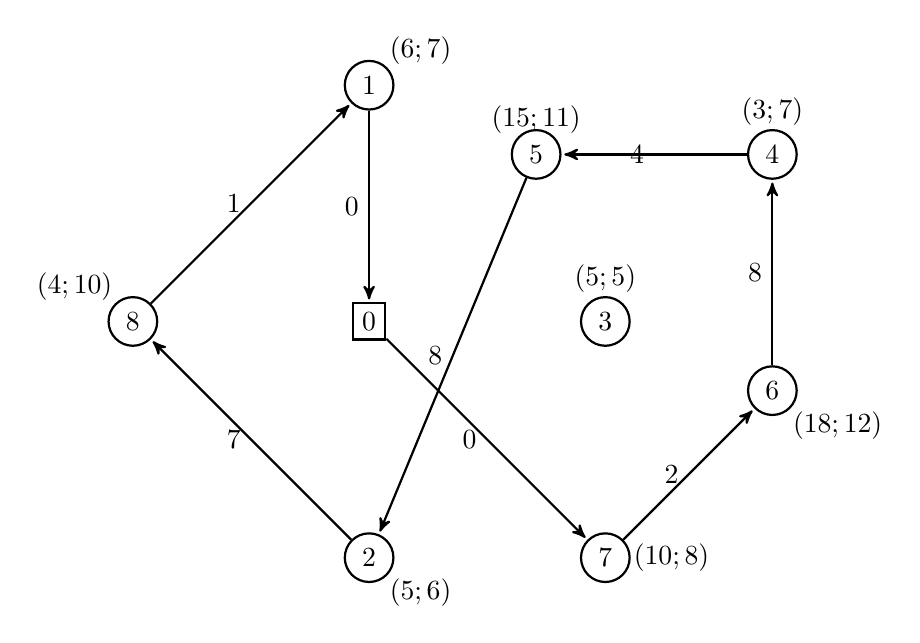
\begin{tikzpicture}[->,>=stealth',shorten >=1pt,auto,node distance=3cm,
                        thick, node/.style={circle,draw}, main node/.style={draw}]
    
      \node[main node] (1) {0};
      \node[node] (2) [above of=1] {1};
      \node[node] (3) [below of=1] {2};
      \node[node] (4) [right of=1] {3};
      \node[node] (5) [above right of=4] {4};
      \node[node] (6) [left of=5] {5};
      \node[node] (7) [below of=5] {6};
      \node[node] (8) [left of=1] {8};
      \node[node] (9) [right of=3] {7};
      
      \extralabel  {45}{\((6; 7)\)}{2};
      \extralabel  [1mm]{90}{\((5; 5)\)}{4};
      \extralabel  [1mm]{90}{\((3; 7)\)}{5};
      \extralabel  {90}{\((15; 11)\)}{6};
      \extralabel  {315}{\((18; 12)\)}{7};
      \extralabel  [1mm]{0}{\((10; 8)\)}{9};
      \extralabel  {315}{\((5; 6)\)}{3};
      \extralabel  {135}{\((4; 10)\)}{8};
    
      \path[every node/.style={}]
        (1) edge node [left] {0} (9)
        (9) edge node [left] {2} (7)
        (7) edge node [left] {8} (5)
        (5) edge node [left] {4} (6)
        (6) edge node [left] {8} (3)
        (3) edge node [left] {7} (8)
        (8) edge node [left] {1} (2)
        (2) edge node [left] {0} (1);
        
    \end{tikzpicture}
    \caption{Exemplo de uma rota viável \cite{art:REF_ART_2}}
    \label{fig:my_label}
\end{figure}
\chapter{Revisão da literatura}\label{chp:LABEL_CHP_2}

\par Neste capítulo, o leitor encontrará sínteses de trabalhos anteriores de autores que estudaram e desenvolveram modelos, exatos ou não, para enfrentar problemas, que aqui foram agrupados se fossem de alguma forma relacionados ao BSS, e tentar resolvê-los. É importante observar que o problema de rebalanceamento de bicicletas nos sistemas de compartilhamento pode ser visto como um problema de otimização combinatória. As diversas categorizações deste problema com relação ao tamanho da frota de veículos, se são permitidas múltiplas visitas às estações e se é permitida a técnica de preempção, foram identificadas como pertencentes ao conjunto dos problemas $\mathcal{NP}$-Hard.

\section{Hernández-Pérez e Salazar-González, 2004}\label{sec:LABEL_CHP_2_SEC_A}

Neste primeiro artigo, os autores não estudaram propriamente o BSS, porém, ele é citado em diversos trabalhos que realmente o analisaram, visto que os conceitos por ele apresentados são muito semelhantes aos do BSS. O objeto de estudo deles foi o Problema do caixeiro viajante de entrega e coleta de um produto, \textit{one-commodity pickup-and-delivery traveling salesman problem - 1-PDTSP}, em inglês, que está intrisecamente ligado ao problema do caixeiro viajante original, \textit{traveling salesman problem - TSP}, em inglês. Por alto, ele possui as seguintes características: cada estação possui uma demanda de entrega ou de coleta de um mesmo produto, o veículo tem uma capacidade máxima de carga determinada, cada estação só pode ser visitada uma vez (em outras palavras, temos um circuito hamiltoniano) e existe uma estação especial chamada de depósito. O objetivo seria encontrar uma rota de custo mínimo, iniciando e finalizando no depósito, que compreendesse todas as estações com ou sem demanda. Ao final, quando o veículo visitasse todas as estações da rota, coletando ou entregando o produto, não mais haveria demanda em nenhuma delas. Cada visita não poderia infringir as capacidades máxima e mínima de carga do veículo. Os estudiosos deste problema construíram um modelo de programação linear inteira e desenvolveram um algoritmo \textit{branch-and-cut} para encontrar uma solução ótima para o modelo proposto, que suportava, em tempo hábil, instâncias do problema com até 60 estações. Deste artigo, diversos autores, inclusive os que serão citados nesse trabalho, utilizam as istâncias descritas nele para a comparação de diversos algoritmos desenvolvidos para resolver não só o 1-PDTSP, como também variações do BSS e do TSP.

\section{Hernández-Pérez, Salazar-González, Rodrígues-Martín, 2008}\label{sec:LABEL_CHP_2_SEC_B}

Os autores do trabalho anterior nesse artigo procuraram outro meio de atacar o problema 1-PDTSP, desta vez com uma tática inexata, utilizando as heurísticas GRASP \citep{resende:1}, \textit{Greedy Randomized Adaptive Search Procedure}, para construção de uma solução inicial, e a VND \citep{art:REF_ART_8}, \textit{Variable Neighborhood Descent}, na itensificação pela busca de outras soluções a partir daquela inicial. Eles compararam essa técnica com a do artigo anterior e os testes realizados com as mesmas instâncias mostraram que a metodologia heurística empregada produziu resultados melhores que as da tática exata. Eles também mostraram que a averiguação da viabilidade de uma solução poderia ser calculada em tempo linear em relação ao número de estações presentes na solução. As vizinhanças utilizadas no procedimento VND foram variações dos operadores 2-opt e 3-opt coletados de \citep{JohnMcGe97} de troca de arestas. Outras duas estruturas de vizinhança foram definidas na fase que os autores nomearam como pós-otimização, na tentativa de melhorar a melhor solução até então escolhida.

\section{Chemla, Meunier, Calvo, 2013}\label{sec:LABEL_CHP_2_SEC_C}

O trabalho dos autores desta seção é o primeiro da lista que já estuda o BSS, abordando o rebalanceamento estático e a permissão da técnica de preempção. Os autores desenvolveram um modelo exato, que logo se mostrou intratável. Eles então relaxaram o modelo, chegando a um problema de programação linear inteira com um número exponencial de restrições, para o qual foi proposto um algoritmo BC,  \textit{branch-and-cut}, como no artigo de \citet{art:REF_ART_3}, para encontrar um limite inferior em relação à solução ótima do problema original. Para traçar os limites superiores do problema, os autores empregaram a busca tabu. Ao longo do trabalho, os autores provam as várias proposições utilizadas por eles no desenvolvimento do algoritmo final, entre as quais vale citar a decisão em tempo polinomial se uma sequência de vértices induz uma solução viável ou não e também, no mesmo tempo algorítmico, as operações possíveis que levam o sistema ao estado mais próximo do objetivo, dada a mesma entrada da proposição anterior.

\section{Paes, Subramanian, Ochi, 2010}\label{sec:LABEL_CHP_2_SEC_D}

Este artigo se trata de outra maneira de lidar com o 1-PDTSP introduzido pelos autores da seção \ref{sec:LABEL_CHP_2_SEC_A} e utiliza heurísticas diferentes das apresentadas na seção \ref{sec:LABEL_CHP_2_SEC_B}, que são o GRASP, o ILS, \textit{Iterated Local Search}, e o RVND, \textit{Random Variable Neighborhood Search}. Além dessas técnicas, os autores ainda implementaram um pré-processamento das instâncias do problema, utilizando 3 restrições que impedem que o espaço de busca inteiro de soluções seja utilizado num primeiro momento na busca por soluções viáveis. O resto desse espaço só é utilizado quando não é possível encontrar um caminho viável utilizando apenas a melhor parte dele. Um exemplo de restrição é a não consideração dos arcos entre as estações que possuem um custo maior que o custo médio entre todos eles. Os autores também desenvolveram uma função de avaliação de inserção de uma estação num caminho corrente que leva em conta o custo entre os arcos e a taxa de violação da carga do veículo. Eles aplicaram 5 estruturas de vizinhança no algortimo RVND e apenas o procedimento \textit{double-bridge} na fase de perturbação. O experimentos realizados, comparados àqueles do trabalho da seção \ref{sec:LABEL_CHP_2_SEC_B}, mostraram que a técnica empregrada obteve desempenho satisfatório nas instâncias pequenas em relação ao tempo, e, quando instâncias de tamanho maior foram utilizadas, ela melhorou as soluções ótimas até então conhecidas na literatura. 

\section{Cruz, Subramanian, Bruck, Iori, 2016}\label{sec:LABEL_CHP_2_SEC_E}

Os autores do artigo desta seção estudaram a mesma variação do BSS da seção \ref{sec:LABEL_CHP_2_SEC_C}, utilizando outras técnicas para trabalhá-lo e analisá-lo. Empregando um modelo inexato, utilizando as herísticas ILS e RVND aliadas aos conceitos desenvolvidos no trabalho da seção já citada, os autores reportaram melhores resultados para o problema. Eles utilizaram 6 estruturas de vizinhança na fase de busca local com o RVND, e 4 procedimentos na fase de perturbação da solução. Além disso, eles perceberam que o processo proposto por \citep{art:REF_ART_2} para verificar em tempo polinomial se uma sequência de vértices induz uma solução viável é custoso, e que em futuros trabalhos pode ser trabalhado e aperfeiçoado. Os autores também analisaram o peso das combinações das perturbações utilizadas no tempo final do algoritmo.

\section{Cruz, Subramanian, Bruck, Iori, 2016}\label{sec:LABEL_CHP_2_SEC_F}

Os mesmos autores do artigo da seção anterior também estudaram o BSS com rebalanceamento estático sem preempção. Eles utilizaram as heurísticas ILS e RVND, contudo, a fase de perturbação da solução ainda emprega a heurística \textit{simulated annealing}, a qual permite que uma solução pior que a já encontrada seja aceita. Os autores deixaram de usar as vizinhas do trabalho anterior que permitiam a técnica de preempção diminuindo para 2 os procedimentos utilizados na perturbação de soluções. Porém, um diferencial em relação ao trabalho predecessor é a utlização de estruturas de dados que permite determinar, em tempo constante, se um movimento numa solução já construída produzirá uma solução viável ou não. Essas estruturas foram primariamente definidas no trabalho que será sumarizado na próxima seção.

\section{Bulhões, Subramanian, Erd\u{o}gan, Laporte, 2016}\label{sec:LABEL_CHP_2_SEC_G}

Diferentemente dos trabalhos anteriores, esta variação estuda o BSS com não apenas um veículo percorrendo as estações, mas vários de igual capacidade. Os autores apresentaram a heurística ILS acompanhada do RVND, como nos trabalhos anteriores, mas também desenvolveram uma formulação de programação linear e um algoritmo BC associado. Nos trabalhos anteriores, o objetivo era encontrar uma rota de custo mínimo, enquanto que neste o objetivo é encontrar uma configuração de rotas, visto que haverá uma rota para cada veículo saindo e retornando ao depósito, de custo mínimo. Algo a ser citado também é a proibição de uma estação ser visitada por veículos diferentes durante o processo. Como dito anteriormente, o trabalho da seção anterior utiliza as estruturas de dados deste artigo para verificar a viabilidade de um movimento em tempo constante sobre uma sequência de vértices. Tais estruturas são de extrema importância, por conta da existência de estruturas de vizinhança numa e entre rotas. Os mecanismos de perturbação também podem ser aplicados entre rotas. Ao final, os autores comparam os resultados entre os métodos heurístico e exato, mostrando que o primeiro teve um desempenho consideravelmente melhor em relação ao segundo.
\chapter{Definição do algoritmo base de comparação}\label{chp:LABEL_CHP_3}

\par Para fins de comparação, será utilizado neste estudo o algoritmo proposto em \citet{art:REF_ART_1}. Ele foi modelado conforme as mesmas características definidas no primeiro capítulo deste. O algoritmo será reproduzido aqui e explicado detalhadamente.
\par Começando pelo algoritmo 1, o procedimento principal. Nele, a heurística ILS é repetida $I_R$ vezes, como pode ser visto na linha 2. Para cada iteração, uma solução $s$ é construída e uma cópia dela é feita, conforme as linhas 3 e 4. Entre as linhas 8 e 19, a heurística \textit{simulated annealing} é executada, decidindo se uma solução $s$ recém-descoberta pelo procedimento RVND deve substituir a solução até então escolhida na iteração $ILS_i$. Em seguida, $s^\lq$ sofre um procedimento de perturbação. Finalmente, ao fim da iteração $i$, a solução $s^*$ é substituída se aquela encontrada pela execução da heurística ILS é melhor do que ela. O custo $f$ de uma solução é dado pela distância necessária para percorrer seu caminho $l$, a saber, $\sum_{i=2}^{n}c_{l_{i-1}},c_{l_i}$.
\par O algoritmo 2 detalha o procedimento de geração de soluções executado na linha 3 do algoritmo 1. Na inicialização dele, temos o preenchimento da variável $Q^\lq$ com a capacidade máxima do veículo, a construção da lista das estações candidatas que estarão na solução $s$, iniciada sempre no depósito. Entre as linhas 6 e 14, temos a escolha da próxima estação que pode ter sua demanda levada a zero em apenas uma visita. Caso não seja possível encontrá-la, entre as linhas 15 e 23 a estação que conceda o maior fechamento de demanda possível é escolhida, seja de entrega ou de coleta. Se for encontrada mais de uma estação com esse valor máximo, aquela esteja mais perto da última adicionada à solução é escolhida. Esse procedimento constrói apenas soluções viáveis. É importante frisar que uma solução é composta por seu custo, caminho, uma sequência de operações realizadas ao longo do caminho e suas estruturas de dados auxiliares, que serão explicadas posteriormente.
\par O algoritmo 3 apresenta o procedimento RVND, como consultado em \citet{art:REF_ART_7}. Ele busca numa lista de vizinhanças pré-definida a melhor solução que pode ser encontrada a partir de uma inicial. As vizinhanças serão definidas posteriormente. O algoritmo 4 elucida os passos da perturbação de uma solução, que utilizada duas vizinhanças que serão abordadas num momento oportuno. Entretanto, pode-se adiantar que a perturbação pode produzir soluções viáveis e inviáveis, ao passo que o procedimento RVND, se receber uma solução viável, sempre retornará outra nestas mesmas condições ou a que foi dada como argumento de entrada, se não houver nenhuma válida que a melhore. Se ele receber uma solução inviável, também será procurada uma que seja viável, retornando aquela provida como entrada se não existir nenhuma que se mostre correta. Graças às estruturas de dados definidas em \citet{art:REF_ART_4}, todos os testes necessários para verificar se uma solução produzida a partir de outra mantém a viabilidade (ou se torna viável) são feitos em tempo constante. Elas serão definidas mais tarde. Ademais, se num caminho de uma solução houver visitas consecutivas a uma mesma estação, elas são unificadas em apenas uma visita, o que pode acontecer na produção de soluções nos procedimentos RVND e no de perturbação.

    \begin{algorithm}[H]
    \caption{ILS-RVND}
    \begin{algorithmic}[1]
    \REQUIRE $I_R \in \mathbb{N}, I_{ILS} \in \mathbb{N}, T \in \mathbb{N}, \alpha \in \mathbb{R}$
    \ENSURE A melhor solução $s^*$ encontrada no procedimento
    \STATE $f^* \leftarrow \infty$
    \FOR{\(i \leftarrow 0\) até \(I_R\)}
        \STATE $s \leftarrow GeraSolucaoInicial$
        \STATE $s^\lq \leftarrow s$
        \STATE $custoAtual \leftarrow f(s)$
        \STATE $iterILS \leftarrow 0$
        \STATE $T \leftarrow T_0$
        \WHILE{$iterILS \leq I_{ILS}$}
            \STATE $s \leftarrow RVND(s, custoAtual)$
            \STATE $\delta \leftarrow f(s) - f(s^\lq)$
            \IF{$\delta < 0$}
                \STATE $s^\lq \leftarrow s$
                \STATE $iterILS \leftarrow 0$
            \ELSE
                \STATE $x \in [0, 1]$
                \IF{$T > 0\; \land\; x < e^{-\delta/T}$}
                    \STATE $s^\lq \leftarrow s$
                \ENDIF
            \ENDIF
            \STATE $s \leftarrow perturba(s^\lq)$
            \STATE $custoAtual \leftarrow f(s)$
            \STATE $iterILS \leftarrow iterILS + 1$
            \STATE $T \leftarrow T \times \alpha$
        \ENDWHILE
        \IF{$f(s^\lq) < f^*$}
            \STATE $s^* \leftarrow s^\lq$
            \STATE $f^* \leftarrow f(s^\lq)$
        \ENDIF
    \ENDFOR
    \RETURN $s^*$
    \end{algorithmic}
    \end{algorithm}
    
    \begin{algorithm}[H]
    \caption{Gera Solucão Inicial}
    \begin{algorithmic}[1]
    \STATE $Q\lq \leftarrow Q$
    \STATE $s \leftarrow \{0\}$
    \STATE $OV \leftarrow $ \{Todas as estações que possuem demanda seguindo uma ordem aleatória\} $\cup$ \{Estações que não possuem demanda escolhidas aleatoriamente\}
    \REPEAT
        \STATE $inseriu \leftarrow \FALSE$
        \FORALL{$i \in OV$}
            \IF{(\,$d_i \leq 0\; \land\; \left|d_i\right| \leq Q^\lq)\,
                \lor (\,d_i > 0\; \land\; Q-Q^\lq \geq d_i)\,$}
                \STATE $s \leftarrow s \cup \{i\}$
                \STATE $Q^\lq \leftarrow Q^\lq + d_i$
                \STATE Retire $i$ de $OV$
                \STATE $inseriu \leftarrow \TRUE$
                \STATE $break$
            \ENDIF
        \ENDFOR
        \IF{$inseriu = \FALSE$}
            \FORALL{$j \in OV$}
                \STATE $calcule troca_j$
            \ENDFOR
            \STATE $c \leftarrow max\{troca_j\; \;|\; \;j \in troca\}$
            \STATE $s \leftarrow s \cup \{c\}$
            \STATE Atualize $d_i$
            \STATE Atualize $Q^\lq$
        \ENDIF
    \UNTIL{$OV \neq \emptyset$}
    \STATE $s \cup \{0\}$
    \RETURN $s$
    \end{algorithmic}
    \end{algorithm}
    
    \begin{algorithm}[H]
    \caption{RVND}
    \begin{algorithmic}[1]
    \REQUIRE Solução $s$
    \ENSURE A melhor solução $s^*$ encontrada na busca
    \STATE Inicializar lista de vizinhanças $LN$
    \STATE $s^* \leftarrow s$
    \WHILE{$LN \neq \emptyset$}
        \STATE Escolha uma vizinhança $N \in LN$ aleatoriamente
        \STATE Encontre o melhor vizinho $s^\lq$ de $s^* \in N$
        \IF{$f(\,s^\lq)\, < f(\,s^*)\,$}
            \STATE $s^* \leftarrow s^\lq$
        \ELSE
            \STATE Remova $N$ de $LN$
        \ENDIF
    \ENDWHILE
    \RETURN $s^*$
    \end{algorithmic}
    \end{algorithm}
    
    \begin{algorithm}[H]
    \caption{perturba}
    \begin{algorithmic}[1]
    \REQUIRE Solução $s$
    \ENSURE Uma solução $s$ que sofreu uma perturbação
    \STATE $i \in [0,1]$
    \IF{$i = 0$}
        \RETURN $doubleBridge(s)$
    \ELSE
        \RETURN $splitP(s)$
    \ENDIF
    \end{algorithmic}
    \end{algorithm}
\chapter{Auxiliary Data Structures}\label{chp:LABEL_CHP_4}
\par Neste capítulo será apresentada a estrutura de dados definida em \citet{art:REF_ART_4}, que foi baseada nos conceitos e ideias apontados por \citet{art:REF_ART_3}, utilizada para melhorar as heurísticas utilizadas em \citet{art:REF_ART_1} com o intuito de diminuir o esforço computacional, o tempo de execução do algoritmo e, em especial, os testes necessários para verificar se um movimento de uma vizinhança sobre o caminho de uma solução produz uma que seja viável.

\section{Definição das ADSs}\label{sec:LABEL_CHP_4_SEC_A}
\par Seja $\sigma = (\, \sigma_{(\,0)\,}, \sigma_{(\,1)\,}, ..., \sigma_{(\,|\sigma| - 1)\,})\,$ uma subsequência do caminho de uma solução S e $\overleftarrow{\sigma}$ a subsequência associada ao caminho inverso dela. Seja também $\sigma_{i, j}$ a subsequência de $\sigma$ que começa na posição $i$ e termina na posição $j$, ou seja, $\sigma_{i, j} = (\, \sigma_{(\,i)\,}, ..., \sigma_{(\,j)\,})\,$. Finalmente, seja $q^{\lq}_{\sigma_{(\,i)\,}}$ a quantidade de bicicletas entregues ou coletadas na visita à estação $i$. A partir dessas variáveis, temos outras que podem ser vistas abaixo:

    \begin{itemize}
        \item $q_{sum}(\,\sigma)\, = \sum^{|\sigma|-1}_{i=0}q^{\lq}_{\sigma_{(\,i)\,}}$, que se constitui pela soma cumulativa de cargas entregues e coletadas;
        \item $q_{min}(\,\sigma)\, = min\{0, q_{sum}(\,\sigma_{0, 0})\,, q_{sum}(\,\sigma_{0, 1})\, ..., q_{sum}(\,\sigma_{0, |\sigma|-1})\,\}$ que acaba por ser a menor carga acumulada na sequência;
        \item $q_{max}(\,\sigma)\, = max\{0, q_{sum}(\,\sigma_{0, 0})\,, q_{sum}(\,\sigma_{0, 1})\, ..., q_{sum}(\,\sigma_{0, |\sigma|-1})\,\}$ que é a carga máxima acumulada;
        \item $l_{min}(\,\sigma)\, = -q_{min}(\,\sigma)\,$ que é o fluxo mínimo de carga que pode entrar na sequência a fim de manter a sua viabilidade (ou para evitar que a inviabilidade cresça);
        \item $l_{max}(\,\sigma)\, = Q -q_{max}(\,\sigma)\,$ que é o fluxo máximo de carga que pode entrar na sequência a fim de manter a sua viabilidade (ou para evitar que a inviabilidade cresça).
    \end{itemize}
    
\par Felizmente, todas as variáveis citadas acima podem ser calculadas em tempo constante para a sequência inversa $\overleftarrow{\sigma}$, fazendo desnecessário o seu armazenamento. O modo de cálculá-las segue adiante:

    \begin{itemize}
        \item $q_{sum}(\,\overleftarrow{\sigma})\, = q_{sum}(\,\sigma)\,$;
        \item $q_{min}(\,\overleftarrow{\sigma})\, = q_{sum}(\,\sigma)\, - q_{max}(\,\sigma)\,$;
        \item $q_{max}(\,\overleftarrow{\sigma})\, = q_{sum}(\,\sigma)\, - q_{min}(\,\sigma)\,$;
        \item $l_{min}(\,\overleftarrow{\sigma})\, = -q_{sum}(\,\sigma)\, + q_{max}(\,\sigma)\,$;
        \item $l_{max}(\,\overleftarrow{\sigma})\, = Q -q_{sum}(\,\sigma)\, + q_{min}(\,\sigma)\,$ .
    \end{itemize}
    
\par Além dos cálculos em tempo constante das variáveis em relação ao caminho inverso, também foi definido o operador $\oplus$, que se refere à concatenação de duas subsequências quaisquer. Para a concatenação de duas subsequências, todas as variáveis anteriores podem ser computadas em tempo constante de acordo com as equações abaixo:

    \begin{itemize}
        \item $q_{sum}(\,\sigma^1 \oplus \sigma^2)\, = q_{sum}(\,\sigma^1)\, + q_{sum}(\,\sigma^2)\,$;
        \item $q_{min}(\,\sigma^1 \oplus \sigma^2)\, = min\{q_{min}(\,\sigma^1)\,, q_{sum}(\,\sigma^1)\, + q_{min}(\,\sigma^2)\,\}$;
        \item $q_{max}(\,\sigma^1 \oplus \sigma^2)\, = max\{q_{max}(\,\sigma^1)\,, q_{sum}(\,\sigma^1)\, + q_{max}(\,\sigma^2)\,\}$;
        \item $l_{min}(\,\sigma^1 \oplus \sigma^2)\, = -q_{min}(\,\sigma^1 \oplus \sigma^2)\,$;
        \item $l_{max}(\,\sigma^1 \oplus \sigma^2)\, = Q - q_{max}(\,\sigma^1 \oplus \sigma^2)\,$ .
    \end{itemize}
    
\par O total de subsequências de uma solução $S$ é da ordem de $|V|^2$, o que significa que a atualização de todas as ADSs de uma solução possui cerca de $O(\,|V|^2)\,$ operações. Algumas observações sobre viabilidade de uma solução podem ser feitas utilizando os cálculos supracitados. Dada uma subsequência qualquer, ela será viável se o valor $l_{min}$ associado a ela é zero, ou seja, o valor mínimo de carga que pode entrar na solução para mantê-la viável é nulo, e o valor $l_{max}$ não pode ser negativo, visto que dessa forma haveria um fluxo $q_{max}$ maior que a capacidade máxima $Q$ do veículo em alguma visita na subsequência. Dadas duas subsequências arbitrárias, $\sigma^1$ e $\sigma^2$, a concatenação delas só será viável se os valores associados à primeira subsequência obedecem as regras introduzidas na observação anterior. E ainda, o valor $q_{sum}(\,\sigma^1)\,$ deve ser maior ou igual a $l_{min}(\,\sigma^2)\,$ e menor ou igual a $l_{max}(\,\sigma^2)\,$.

\section{Construindo as ADSs}\label{sec:LABEL_CHP_4_SEC_B}

\par As ADSs podem ser armazenadas utilizando um vetor bidimensional, uma matriz, de valores inteiros. É importante notar que tal matriz é triangular superior, por conta de não são realizadas consultas de subsequências $\sigma_{i,j}$ com $i > j$. O algoritmo 5 descreve os passos para a construção das ADSs de uma solução $S$. As linhas 3 e 12 mostra que a operação feita na visita à estação $i$ tem seu sinal trocado. Observe que o primeiro laço de repetição começa com $i=1$, visto que a operação feita no índice zero do caminho de $S$ é nula, tendo em vista que nada é feito ao sair do depósito. Assim, os valores relacionados a $\sigma_{0, 0}$ de qualquer $\sigma$ são $q_{sum} = q_{min} = q_{max} = l_{min} = 0$ e $l_{max} = Q$. O algoritmo de construção das ADSs pode ser facilmente adaptado para apenas atualizar os valores de uma pedaço com início $a$ e final $b$ de uma subsequência de $\sigma$. Nesse caso, as ADSs associadas às subsequências $\sigma_{i, j}$ com $i < a \land j < a$ ou com $i > b \land j > b$ não precisam ser recalculadas. Para deixar de cálculá-las començamos substituindo o valor máximo de $i$ no bloco \textit{para} da linha 2 por $j$. Então, precisamos tratar dois casos do loop 2, os quais são:
    
    \begin{itemize}
        \item $i < a$: Os valores da ADS de $\sigma_{i, a}$ são calculados como se segue:
        \begin{enumerate}
            \item $q_{sum}(\,\sigma_{i, a})\, = q_{sum}(\,\sigma_{i, a-1})\, + g_a$
            \item $q_{min}(\,\sigma_{i, a})\, = min\{q_{sum}(\,\sigma_{i, a})\,, q_{sum}(\,\sigma_{i, a-1})\,\}$
            \item $q_{max}(\,\sigma_{i, a})\, = max\{q_{sum}(\,\sigma_{i, a})\,, q_{sum}(\,\sigma_{i, a-1})\,\}$
            \item O valor inicial de $j$ no laço da linha 11 é $a + 1$
        \end{enumerate}
        \item $i \geq a$: os valores são calculados utilizando somente $g_i$ e o valor de $j$ no laço da linha 11 é $i + 1$.
    \end{itemize}
    
\par Tomando como exemplo o caminho da figura \ref{fig:my_label} de $n = Q = 8$ e operações \( g = <0, +2, +6, -4, +4, -1, -6, -1>\), teríamos $q_{sum}(\,\sigma)\, = 0\; +\; 2\; +\; 6\; -\; 4\; +\; 4\; -\; 1\; -\; 6\; -\; 1 = 0$, $q_{min}(\,\sigma)\, = min\{0, 2, 8, 4, 8, 7, 1, 0\} = 0$, $q_{max}(\,\sigma)\, = max\{0, 2, 8, 4, 8, 7, 1, 0\} = 8$, $l_{min}(\,\sigma)\, = 0$ e $l_{max}(\,\sigma)\, = 8 - 8 = 0$. Agora, fazendo os cálculos apenas sobre a subsequência $\sigma_{(\,3, 5)\,} = \{4, 5, 2\}$, temos $q_{sum}(\,\sigma_{(\,3, 5)\,})\, = -\; 4\; +\; 4\; -\; 1\; = -1$, $q_{min}(\,\sigma_{(\,3, 5)\,})\, = min\{0, -4, 0, -1\} = -4$, $q_{max}(\,\sigma_{(\,3, 5)\,})\, = max\{0, -4, 0, -1\} = 0$, $l_{min}(\,\sigma_{(\,3, 5)\,})\, = 4$ e $l_{max}(\,\sigma_{(\,3, 5)\,})\, = 8 - 4 = 4$.

    \begin{algorithm}[H]
    \caption{Construir ADS}
    \begin{algorithmic}[1]
    \REQUIRE Solução $s$, $Q \in \mathbb{N}$
    \ENSURE As estruturas auxiliares de dados de $s$ são inicializadas
    \STATE $ADS \leftarrow$ Matriz de dimensões $N \times N$, em que N é o tamanho do caminho de $s$
    \FOR{$i=1$ até $N$}
        \STATE $q_{sum} \leftarrow g_i$
        \STATE $q_{min} \leftarrow min\{0, q_{sum}\}$
        \STATE $q_{max} \leftarrow max\{0, q_{sum}\}$
        \STATE $ADS[i, i].q_{sum} \leftarrow q_{sum}$
        \STATE $ADS[i, i].q_{min} \leftarrow q_{min}$
        \STATE $ADS[i, i].q_{max} \leftarrow q_{max}$
        \STATE $ADS[i, i].l_{min} \leftarrow -q_{min}$
        \STATE $ADS[i, i].l_{max} \leftarrow Q - q_{max}$
        \FOR{$j = i + 1$ até $N$}
            \STATE $q_{sum} \leftarrow q_{sum} + g_j$
            \STATE $q_{min} \leftarrow min\{q_{sum}, q_{min}\}$
            \STATE $q_{max} \leftarrow max\{q_{sum}, q_{max}\}$
            \STATE $ADS[i, j].q_{sum} \leftarrow q_{sum}$
            \STATE $ADS[i, j].q_{min} \leftarrow q_{min}$
            \STATE $ADS[i, j].q_{max} \leftarrow q_{max}$
            \STATE $ADS[i, j].l_{min} \leftarrow -q_{min}$
            \STATE $ADS[i, j].l_{max} \leftarrow Q - q_{max}$
        \ENDFOR
    \ENDFOR
    \end{algorithmic}
    \end{algorithm}
\chapter{Estruturas de vizinhança}\label{chp:LABEL_CHP_5}

\par Neste capítulo serão tratadas as estruturas de vizinhança utilizadas nos procedimentos RVND e de perturbação. Ela consiste de um determinado movimento feito sobre uma solução, testando-se todas as possibilidades, a fim de encontrar uma que seja a mais proveitosa que, neste caso, é a que possui um menor custo e que ainda seja viável. Os custos entre as arestas que serão utilizados para calcular o custo final dos vários exemplos que serão feitos são oriundos da instância \textit{n20q10A.tsp} definida em \citep{art:REF_ART_3} e reutilizada em \citep{art:REF_ART_5}.

\section{Vizinhanças da busca local}\label{sec:LABEL_CHP_5_SEC_A}

\par Nesta seção serão apresentadas as vizinhanças utilizadas no procedimento RVND, que como já dito, sempre retorna soluções viáveis ou aquela dada como argumento de entrada se não houver nenhuma solução válida que a melhore.

\subsection{2-OPT}\label{sec:LABEL_CHP_5_SUBSEC_A}

\par O movimento desta vizinhança é bastante simples: dadas duas posições $i$ e $j$ de um caminho qualquer, com $j > i + 2$, a subsequência entre esses pontos é invertida. Assim, o objetivo é encontrar essas duas posições que resultem numa subsequência 
    
    \begin{gather}
        \sigma^\lq = \sigma_{(\,0, i)\,}\; \oplus\; \overleftarrow{\sigma}_{(\,i+1, j-1)\,}\; \oplus\; \sigma_{(\,j, |\sigma|-1)\,}
    \end{gather}
    
que seja viável e tenha um custo $f(\,\sigma^\lq)\, < f(\,\sigma)\,$. Sabendo que além do custo de $\sigma$ ser conhecido, também é sabido o custo $c_{(\,a, b)\,} \forall\; a, b \in V$, assim, é possível saber o custo do novo caminho em tempo constante sem a necessidade de calculá-lo do zero. Este custo se dá por:

    \begin{gather}
        f(\,\sigma^\lq)\, = f(\,\sigma)\, - (\,c_{(\,i, i+1)\,} + c_{(\,j-1, j)\,})\, + (\,c_{(\,i, j-1)\,} + c_{(\,i+1, j)\,})\,
    \end{gather}
    
sendo $i$ e $j$ vértices nas posições $i$ e $j$ do caminho da solução. A sequência de operações associada ao pedaço que será invertido deve sofrer a mesma operação para que continue a caracterizar o caminho representado pela solução. Para fins de exemplificação, usemos o caminho apresentado na figura \ref{fig:my_label} e tomemos $i = 0$ e $j = 5$. Para verificar se essa é uma operação possível, devemos nos atentar às ADSs associadas às subsequências $\sigma_{(\,0, 0)\,}$, $\sigma_{(\,1, 4)\,}$ e $\sigma_{(\,5, 8)\,}$.

\par Sabendo que $q_{sum}(\,\sigma_{(\,0, 0)\,})\, = 0$ é maior ou igual a $l_{min}(\,\overleftarrow{\sigma}_{(\,1, 4)\,})\, = 0$ e menor ou igual a $l_{max}(\,\overleftarrow{\sigma}_{(\,1, 4)\,})\, = 0$, é possível realizar a concatenação dessas subsequências. Ao concatená-las, temos que $q_{sum}(\,\sigma_{(\,0, 0)\,} \oplus \overleftarrow{\sigma}_{(\,1, 4)\,})\,)\, = 0 + 8 = 8$ que é maior ou igual a $l_{min}(\,\sigma_{(\,5, 8)\,})\, = 8$ e menor ou igual a $l_{max}(\,\sigma_{(\,5, 8)\,})\, = 8$, o que nos leva a concluir que o movimento analisado é válido. O custo do caminho produzido pelo movimento, tendo em vista que $f(\,\sigma)\, = 3899,\; c_{(\,0, 1)\,} = 418,\; c_{(\,4, 5)\,} = 274,\; c_{(\,0, 4)\,} = 123$ e $c_{(\,1, 5)\,} = 183$, conduz a $f(\,\sigma^\lq)\, = 3513$, melhorando o custo da solução de exemplo.

\subsection{Swap}\label{sec:LABEL_CHP_5_SUBSEC_B}

\par Esta vizinhança se caracteriza pelo seguinte movimento: dadas duas posições $i$ e $j$ de um caminho qualquer, com $j > i$, os vértices nessas posições são trocados, isto é, $\sigma_{(\,i, i)\,} \Longleftrightarrow \sigma_{(\,j, j)\,}$. Portanto, o objetivo é encontrar essas duas posições que resultem numa subsequência

    \begin{gather} \label{swapeq:1}
        \sigma^\lq = \sigma_{(\,0, i - 1)\,}\; \oplus\; \sigma_{(\,j, j)\,}\; \oplus\; \sigma_{(\,i+1, j-1)\,}\; \oplus\; \sigma_{(\,i, i)\,}\;
        \oplus\; \sigma_{(\,j+1, |\sigma| - 1)\,}\;
    \end{gather}
    
que seja viável e tenha um custo $f(\,\sigma^\lq)\, < f(\,\sigma)\,$. É importante notar que se $j = i + 1$, a subsequência $\sigma_{(\,i+1, j-1)\,}$ não existirá e teremos:

    \begin{gather} \label{swapeq:2}
        \sigma^\lq = \sigma_{(\,0, i - 1)\,}\; \oplus\; \sigma_{(\,j, j)\,}\;  \oplus\; \sigma_{(\,i, i)\,}\;
        \oplus\; \sigma_{(\,j+1, |\sigma| - 1)\,}\;
    \end{gather}

Podemos calcular o novo custo em tempo constante para o caso \ref{swapeq:1} a partir de:

    \begin{gather} 
    \begin{split}
        f(\,\sigma^\lq)\,& = f(\,\sigma)\, + (\,c_{(\,i-1, j)\,} + c_{(\,j, i+1)\,} + c_{(\,j-1, i)\,} + c_{(\,i, j+1)\,})\, -\\
                         & \quad (\,c_{(\,i-1, i)\,} +       c_{(\,i, i+1)\,} + c_{(\,j-1, j)\,} + c_{(\,j, j+1)\,})\,
    \end{split}
    \end{gather}
    
E para \ref{swapeq:2} teremos:

    \begin{gather}
        f(\,\sigma^\lq)\, = f(\,\sigma)\, + (\,c_{(\,i-1, j)\,}  + c_{(\,i, j+1)\,})\, - (\,c_{(\,i-1, i)\,} + c_{(\,j, j+1)\,})\,
    \end{gather}

Vamos agora aplicar um exemplo com $i=4$ e $j=5$ no caminho da figura \ref{fig:my_label}. Como será reproduzido o caso \ref{swapeq:2}, iremos nos atentar às ADSs associadas às subsequências $\sigma_{(\,0, 3)\,}$, $\sigma_{(\,5, 5)\,}$, $\sigma_{(\,4, 4)\,}$ e $\sigma_{(\,6, 8)\,}$. Primeiramente, notemos que $q_{sum}(\,\sigma_{(\,0, 3)\,})\, = 4 \geq l_{min}(\,\sigma_{(\,5, 5)\,})\, = 1$ e $q_{sum}(\,\sigma_{(\,0, 3)\,})\, = 4 \leq l_{max}(\,\sigma_{(\,5, 5)\,})\, = 8$, o que nos permite concatenar essas duas primeiras subsequências. Assim, prosseguimos com $q_{sum}(\,\sigma_{(\,0, 3)\,} \oplus \sigma_{(\,5, 5)\,})\, = 4 + (\,-1)\, = 3$, que está no intervalo $0 = l_{min}(\,\sigma_{(\,4, 4)\,})\, \leq 3 \leq 4 = l_{max}(\,\sigma_{(\,4, 4)\,})\,$, que nos permite chegar a $q_{sum}(\,\sigma_{(\,0, 3)\,} \oplus \sigma_{(\,5, 5)\,} \oplus \sigma_{(\,4, 4)\,})\, = 4 + (\,-1)\, + 4 = 7$. Finalmente, sabemos que $7 = l_{min}(\,\sigma_{(\,6, 8)\,})\, \leq 7 \leq 8 = l_{max}(\,\sigma_{(\,6, 8)\,})\,$, que nos permite dizer que o movimento inspecionado é válido.

\par O custo do caminho produzido pelo movimento, tendo em vista que $f(\,\sigma)\, = 3899,\; c_{(\,3, 5)\,} = 198,\; c_{(\,4, 6)\,} = 321,\; c_{(\,3, 4)\,} = 337$ e $c_{(\,5, 6)\,} = 568$, conduz a $f(\,\sigma^\lq)\, = 3513$, melhorando o custo da solução de exemplo.

\subsection{or-OPT-k}\label{sec:LABEL_CHP_5_SUBSEC_C}

\par Esta seção trata de quatro movimentos que foram aqui reunidos por apresentarem a mesma ideia. Dadas duas posições $i$ e $j$, deseja-se retirar um número determinado de vértices começando de $i$ para inserí-los após a posição $j$, a saber, $j+1$. O total de vértices a ser movido dita qual é a vizinhança a qual nos referimos. O número $k \in \{1, 2, 3, 4\}$ indica tal quantidade, sendo $k=1$ também conhecido como \textit{reinserção}. Caso $i < j$, é necessário que $j-i >= k + 1$, ou seja, deve haver vértices suficientes para que a tranferência seja feita. E também deve-se garantir que $i > j + 1$ para que haja algum movimento a ser realizado. Similarmente às vizinhanças predecessoras, o objetivo é encontrar essas duas posições que resultem numa sequência
    
    \begin{numcases}{\sigma^\lq =}
      \sigma_{(\,0, i - 1)\,}\; \oplus\; \sigma_{(\,i+k, j)\,}\; \oplus\; \sigma_{(\,i, i+k-1)\,}\; \oplus\; \sigma_{(\,j+1, |\sigma| - 1)\,}, & se $i<j$ \\
      \sigma_{(\,0, j)\,}\; \oplus\; \sigma_{(\,i, i+k-1)\,}\; \oplus\; \sigma_{(\,j+1, i-1)\,}\; \oplus\; \sigma_{(\,i+k, |\sigma| - 1)\,}, & se não
    \end{numcases}
    
que seja viável e tenha um custo $f(\,\sigma^\lq)\, < f(\,\sigma)\,$. O custo pode ser calculado para os dois casos da seguinte forma:

    \begin{gather}
        \begin{split}
        f(\,\sigma^\lq)\, = & f(\,\sigma)\, - (\,c_{(\,i-1, i)\,}  + c_{(\,i+k-1, i+k)\,} + c_{(\,j, j+1)\,})\, +\\ & (\,c_{(\,i-1, i+k)\,} + c_{(\,j, i)\,} + c_{(\,i+k-1, j+1)\,})\,
        \end{split}
    \end{gather}

Agora, vamos aplicar um exemplo com $k=2$, $i=3$ e $j=5$ sobre o caminho da figura \ref{fig:my_label}. Como $i<j$, devemos nos atentar às ADSs associadas às subsequências $\sigma_{(\,0, 2)\,}$, $\sigma_{(\,5, 5)\,}$, $\sigma_{(\,3, 4)\,}$ e $\sigma_{(\,6, 8)\,}$. Começamos descobrindo que $q_{sum}(\,\sigma_{(\,0, 2)\,})\, = 8$, que é maior que $l_{min}(\,\sigma_{(\,5, 5)\,})\, = 1$ e igual a $l_{max}(\,\sigma_{(\,5, 5)\,})\, = 8$. Assim, concatenando essas subsequências, temos $q_{sum}(\,\sigma_{(\,0, 2)\,} \oplus\, \sigma_{(\,5, 5)\,})\, = 8 + (\,-1)\, = 7$, que nos permite verificar que é maior que $l_{min}(\,\sigma_{(\,3, 4)\,})\, = 4$ e menor que $l_{max}(\,\sigma_{(\,3, 4)\,})\, = 8$. Realizando a concatenação, acabamos em $q_{sum}(\,\sigma_{(\,0, 2)\,} \oplus\, \sigma_{(\,5, 5)\,} \oplus\, \sigma_{(\,3, 4)\,})\, = 8 + (\,-1)\, + 0 = 7$. Por último, as últimas condições de concatenação são satisfeitas: $7 \geq l_{min}(\,\sigma_{(\,6, 8)\,})\, = 7$ e $7 \leq l_{max}(\,\sigma_{(\,6, 8)\,})\, = 8$, provando que o movimento sugerido é válido. O custo do caminho resultante, sabendo que $f(\,\sigma)\, = 3899,\; c_{(\,2, 3)\,} = 521,\; c_{(\,4, 5)\,} = 274,\; c_{(\,5, 6)\,} = 568, c_{(\,2, 5)\,} = 701, c_{(\,5, 3)\,} = 198$ e $c_{(\,4, 6)\,} = 321$, conduz a $f(\,\sigma^\lq)\, = 3756$, melhorando o custo da solução de exemplo.

\subsection{Split}\label{sec:LABEL_CHP_5_SUBSEC_D}

\par Falemos agora sobre a última vizinhança da busca local. Durante o caminho de uma solução, consideremos qualquer visita a uma estação cuja operação tenha sido de entrega ou de coleta, mas que tenha envolvido mais de uma bicicleta. Esta visita é fracionada da seguinte forma: uma e somente uma bicicleta envolvida na operação é removida e inserida em outro ponto do caminho, produzinho uma nova visita à estação cuja operação envolva um único produto. Assim, dadas duas posições $i$ e $j$, com $i \neq j$, o objetivo é encontrar uma subsequência

    \begin{numcases}{\sigma^\lq =}
      \sigma_{(\,0, i - 1)\,}\; \oplus\; \sigma_{(\,i, i)\,}^{-1}\; \oplus\; \sigma_{(\,i+1, j-1)\,}\; \oplus\; \sigma_{(\,i, i)\,}^1
      \oplus\; \sigma_{(\,j, |\sigma| - 1)\,}, & se $i<j$ \\
      \sigma_{(\,0, j-1)\,}\; \oplus\; \sigma_{(\,i, i)\,}^1\;  \oplus\; \sigma_{(\,j, i-1)\,}\; \oplus\; \sigma_{(\,i, i)\,}^{-1}\;
      \oplus\; \sigma_{(\,i+1, |\sigma| - 1)\,}, & se não
    \end{numcases}
    
que seja viável e tenha um custo $f(\,\sigma^\lq)\, < f(\,\sigma)\,$. O termo $\sigma_{(\,i,i)\,}^1$ representa a operação unitária sobre uma bicicleta, seja ela de coleta ou entrega, ao passo que $\sigma^{-1}_{(\,i, i)\,}$ se refere à transação com a perda (ou ganho) de menos um produto, cada um em relação à subsequência $\sigma_{(\,i,i)\,}$. Como o custo para visitar uma estação a partir da mesma é zero, não é permitido que $\sigma_{(\,i,i)\,}=\sigma_{(\,j, j)\,}$, $\sigma_{(\,i,i)\,}=\sigma_{(\,j-1, j-1)\,}$ e $\sigma_{(\,i-1,i-1)\,}=\sigma_{(\,j, j)\,}$. O custo pode ser calculado da forma que se segue

    \begin{gather}
        f(\,\sigma^\lq)\, = f(\,\sigma)\, + (\,c_{(\,j-1, i)\,}  + c_{(\,i, j)\,})\, - c_{(\,j-1, j)\,}
    \end{gather}
    
\par Para fins de exemplificação, tomemos $i=1$ e $j=4$ e o caminho da figura \ref{fig:my_label}. Por conta das posições escolhidas, devemos nos ater às ADSs associadas às subsequências $\sigma_{(\,0, 0)\,}$, $\sigma_{(\,1, 1)\,}^{-1}$, $\sigma_{(\,2, 3)\,}$, $\sigma_{(\,1, 1)\,}^1$ e $\sigma_{(\,4, 8)\,}$, visto que $i<j$. Sabemos que a operação feita na visita à estação representada pela subsequência $\sigma_{(\,1, 1)\,}$ é de coleta. Assim, calculemos as informações necessárias: $q_{sum}(\,\sigma_{(\,i, i)\,}^{-1})\, = 2 - 1 = 1$, $l_{min}(\,\sigma_{(\,i, i)\,}^{-1})\, = 0$, $l_{max}(\,\sigma_{(\,i, i)\,}^{-1})\, = 8 - 1 = 7$, $q_{sum}(\,\sigma_{(\,i, i)\,}^{1})\, = 1$, $l_{min}(\,\sigma_{(\,i, i)\,}^{1})\, = 0$ e $l_{max}(\,\sigma_{(\,i, i)\,}^{1})\, = 8 - 1 = 7$. Agora podemos prosseguir, concluindo que $q_{sum}(\,\sigma_{(\,0, 0)}\,)\, = 0$ é igual a $l_{min}(\,\sigma_{(\,0, 0)}^{-1})\,$ e menor que $l_{max}(\,\sigma_{(\,0, 0)})\,$. Podemos então concatenar essas duas subsequências, chegando a $q_{sum}(\,\sigma_{(\,0, 0)\,} \oplus \sigma_{(\,1, 1)\,}^{-1})\, = 0 + 1 = 1$, que é maior que $l_{min}(\,\sigma_{(\,2, 3)})\, = 0$ e menor que $l_{max}(\,\sigma_{(\,2, 3)})\, = 2$. Prosseguimos então com $q_{sum}(\,\sigma_{(\,0, 0)\,} \oplus\, \sigma_{(\,1, 1)\,}^{-1}\, \oplus\, \sigma_{(\,2, 3)})\, = 0 + 1 + 2 = 3$, maior e menor que $l_{min}(\,\sigma_{(\,i, i)\,}^{1})\,$ e $l_{max}(\,\sigma_{(\,i, i)\,}^{1})\,$, respectivamente. Fazendo $q_{sum}(\,\sigma_{(\,0, 0)\,} \oplus\, \sigma_{(\,1, 1)\,}^{-1}\, \oplus\, \sigma_{(\,2, 3)} \oplus\, \sigma_{(\,1, 1)\,}^{-1})\, = 0 + 1 + 2 + 1 = 4$, que, finalmente, é igual a $l_{min}(\,\sigma_{(\,4, 8)})\, = l_{max}(\,\sigma_{(\,4, 8)})\, = 4$. Assim sendo, o movimento realizado é válido. O custo pode ser calculado a partir dos seguintes valores $f(\,\sigma)\, = 3899,\; c_{(\,3, 1)\,} = 223,\; c_{(\,1, 4)\,} = 452$ e $c_{(\,3, 4)\,} = 337$, que conduzem a $f(\,\sigma^\lq)\, = 4237$, piorando o custo da solução de exemplo. Quando, mais à frente, forem apresentados os resultados dos experimentos, será falado sobre o desempenho dessa vizinhança, pois, teoricamente, ao adicionar uma visita ao caminho de uma solução, dificilmente seu custo será diminuído.


\section{Vizinhanças de perturbação}\label{sec:LABEL_CHP_5_SEC_B}

\par Nesta seção serão apresentadas as vizinhanças utilizadas no procedimento de perturbação, que possui altas chances de produzir soluções inviáveis.

\subsection{Split-p}\label{sec:LABEL_CHP_5_SUBSEC_E}

\par Essa é igual à vizinhança introduzida na seção \ref{sec:LABEL_CHP_5_SUBSEC_D}. Porém, nenhuma das análises de prevenção contra soluções inviáveis é feita. Assim, basta que a solução produzida tenha um custo menor que o da original.

\subsection{Double Bridge}\label{sec:LABEL_CHP_5_SUBSEC_F}

\par Esta vizinhança, utilizada em \citep{art:REF_ART_1}, porém esmiuçada melhor em \citep{art:REF_ART_7}, promove o seguinte: duas subsequências, de qualquer tamanho, são permutadas, isto é, são colocadas uma no lugar da outra. Desta forma, dadas 4 posições $p_1, p_2, p_3$ e $p_4$, escolhidas aleatoriamente, respeitando as condições $1 \leq p_1 \leq |\sigma| - 5,\, p_1 \leq p_2 \leq |\sigma| - 4,\, p_2 < p_3 \leq |\sigma| - 3$ e $p_3 \leq p_4 \leq |\sigma| - 2$, uma subsequência

    \begin{numcases}{\sigma^\lq =}
    	\begin{split}
      		\sigma_{(\,0, p_1 - 1)\,}\; \oplus\; \sigma_{(\,p_3, p_4)\,}\; \oplus\; \sigma_{(\,p_2 + 1, p_3 - 1)\,}\; \\ \oplus\; \sigma_{(\,p_1, p_2)\,}
      \oplus\; \sigma_{(\,p_4 + 1, |\sigma| - 1)\,} 
      \end{split}, & se $p_3 - p_2 > 1$ \\
      \sigma_{(\,0, p_1 - 1)\,}\; \oplus\; \sigma_{(\,p_3, p_4)\,}\; \oplus\; \sigma_{(\,p_1, p_2)\,} \oplus\; \sigma_{(\,p_4 + 1, |\sigma| - 1)\,}, & se não
    \end{numcases}
    
podendo não ser viável e não tendo um custo menor que o da sequência original. Tal custo pode ser calculado como $f(\sigma^\lq) = f(\sigma) - (c_{(p_1 - 1, p_1)} + c_{(p_4, p_4 + 1)}) + (c_{(p_1 - 1, p_3)} + c_{(p_2, p_4 + 1)})$. Ademais, temos:

    \begin{numcases}{f(\sigma^\lq) = f(\sigma^\lq) -}
    	\begin{split}
        (c_{(p_2, p_2 + 1)} + c_{(p_3 - 1, p_3)}) - \\ (c_{(p_4, p_2 +1)} + c_{(p_3 - 1, p_1)}) \end{split}, & se $p_3 - p_2 > 1$ \\
        (c_{(p_2, p_3)}) - (c_{(p_4, p_1)}, & se não
    \end{numcases}
    
A título de exemplo, atribuamos os sequintes valores $p_1 = 2, p_2 = 3, p_3 = 4$ e $p_4 = 5$. Como $p_3 - p_2= 4 - 3 = 1$ não é maior que $1$, precisamos apenas de $f(\,\sigma)\, = 3899, c_{1, 2} = 733, c_{5, 6} = 568, c_{1, 4} = 452, c_{3, 6} = 658, c_{3, 4} = 337$ e $c_{5, 2} = 701$ para chegar a $f(\,\sigma^lq)\, = 4072$.
\chapter{Proposta de algoritmo para o problema}\label{chp:LABEL_CHP_6}

\par Será definido neste capítulo um novo algoritmo para que seja comparado aquele apresentado no capítulo \ref{chp:LABEL_CHP_3}, que foi modelado de acordo com duas meta-heurísticas, quais sejam a ILS e a SA. Por outro lado, será proposto neste trabalho um que seja estruturado de acordo com os frameworks apontados pela Busca Tabu \citet{glover}.

\section{A Busca Tabu}\label{sec:LABEL_CHP_6_SEC_A}

\par Essa meta-heurística, diferentemente da ILS, para a obtenção de melhores resultados, ancora-se na premissa de que para uma busca ser considerada inteligente, ela deve incorporar uma memória adaptativa, para que haja economia e eficiência ao guiar a busca com informações coletadas durante a sua execução, e ser responsiva, baseando-se na suposição de que uma má estratégia de escolha pode gerar mais informação que uma boa escolha feita de forma aleatória. Assim, esse modelo heurístico permite que boas características de soluções sejam utilizadas ao mesmo tempo que regiões do espaço de busca ainda não visitadas sejam analisadas.

\par Na seção \ref{sec:LABEL_CHP_2_SEC_C} do capítulo \ref{chp:LABEL_CHP_2} pode-se encontrar uma síntese sobre um trabalho que também utilizou a meta-heurística supracitada. O programa produzido em tal pesquisa se utilizou da estrutura de dados \textit{multimap}, que associa um valor a uma chave específica, da linguagem C++ para implementar a memória da Busca Tabu. Tal componente foi implementado para que a seguinte ideia fosse possível: um arco $ab$ qualquer que foi utilizado numa posição $k$ do caminho da última solução encontrada não poderá ser utilizado novamente por um número determinado de iterações. Com isso, diminui-se a probabilidade de se chegar a uma solução já encontrada, visto que os arcos para se chegar a ela são proibidos, possibilitando uma diversificação no processo de investigação de áreas ainda não vistas. A memória que será utilizada no algoritmo a ser proposto utilizará essa mesma ideia, porém, sua implementação não será feita empregando a estrutura de dados mencionada a pouco, pois apesar de fornecer rápido acesso, tal coisa não é feita em tempo constante.

\par A busca local utilizará as mesmas vizinhanças dispostas em \citet{art:REF_ART_1}, assim como o procedimento RVND para a busca local. No entanto, as vizinhanças de perturbação não serão utilizadas, visto que a diversificação da Busca Tabu é feita a partir de uma análise que se permite caminhar por soluções de qualidade inferiores às das melhores encontradas, além de evitar percorrer por áreas percorridas recentemente, ao passo que a meta-heurística ILS modifica a solução atual utilizando movimentos que a levem a uma região um tanto diferente da que fora recentemente observada. Consequentemente, o procedimento RVND teve que sofrer uma pequena adaptação que será detalhada futuramente neste trabalho.

\section{Bitmap}\label{sec:LABEL_CHP_6_SEC_B}

\par Para que a estrutura de dados elaborada neste trabalho seja apresentada, faz-se necessário que o leitor conheça uma estrutura conhecida como mapa de bits, muito utilizada para a representação de conjuntos numéricos sem desperdício de memória e de desempenho. 

\par Um mapa de bits consiste de uma palavra de bits, dependente da arquitetura do computador utilizado, que possui bits ligados ou desligados. Quando empregado para representar conjuntos, um elemento $i$ pertence ao conjunto se o bit na posição $i$ está definido como 1, e 0 em caso contrário. Caso a quantidade de bits da palavra de bits da máquina seja inferior ao número pretendido de elementos que um conjunto precisa armazenar, pode-se utilizar vetores de mapa de bits. Cada posição do vetor é chamada de \textit{naco}, e estes são inicializados com todos os seus bits como $0$.

\par Seja $n$ o tamanho de um conjunto de números naturais $N$ qualquer e $m$ o tamanho da palavra de bits do computador. Logo, o número de nacos necessários para representar $N$ será $\ceil*{\frac{n}{m}}$. Para descobrir o naco ao qual um elemento $i$ pertence, basta fazer $\floor*{\frac{i}{m}}$. Também tem-se que $i \;\%\; m$, no qual o operador $\%$ retorna o resto da divisão de $i$ por $m$, permite descobir o bit do naco ao qual $i$ pertence que deverá ser aceso ou apagado.

\par Para ligar um bit (incluir um elemento $i$ no conjunto), basta descobrir o naco em que se encontra, aqui nomeado como $A$, e então calcular $A = A \;||\; (1 \ll i \;\%\; m)$. Para desligá-lo (excluir um elemento do conjunto), aplica-se $A = A \;\&\; (\sim 1 \ll (i \;\%\; m))$. Para consultar se $i$ pertence ao conjunto, basta descobrir se $(A \;\&\; ( 1 \ll (i \;\%\; m))) \neq 0$.

\par Desta forma, para a implementação da memória da Busca Tabu enunciada no início desse capítulo, será necessário manter um vetor de mapa de bits para cada arco do grafo que modela uma dada instância do problema. Assim, para saber se um arco foi utilizado numa posição $k$ de uma solução recentemente, pode-se verificar se o valor $k$ está presente em seu respectivo conjunto de bits.

\section{Regras tabu para cada vizinhança}\label{sec:LABEL_CHP_6_SEC_C}

\par Antes de expor o algoritmo completo para a Busca Tabu, as regras de aceitação de um movimento para cada vizinhança vistas no capítulo \ref{chp:LABEL_CHP_5} serão acrescentadas de mais algumas verificações. Essas servirão para descobrir se uma aresta que está para ser movida pelo movimento de uma vizinhança foi utilizada recentemente na posição a qual está destinada. Uma subsequência qualquer de tamanho $n$ terá $n-1$ posições válidas de arcos, que podem ser identificados a partir de qualquer subsequência de dois vértices consecutivos. A seguir constam as novas apurações a serem feitas para cada vizinhança, exceto as de perturbação, que não foram utilizadas no algoritmo proposto.


\subsection{2-OPT}\label{sec:LABEL_CHP_5_SUBSEC_A}

\par Essa vizinhança inverte uma subsequência de vértices entre as posições $i$ e $j$.  Assim, os seguintes arcos não poderão ter sido usados nas seguintes posições recentemente:

	\begin{itemize}
        \item $\sigma_{(i, i)}\sigma_{(j-1, j-1)}$ na posição $i$;
        \item $\sigma_{(i+1, i+1)}\sigma_{(j, j)}$ na posição $j$.
    \end{itemize}
    
\subsection{Swap}\label{sec:LABEL_CHP_5_SUBSEC_B}

\par A vizinhança dessa seção permuta os vértices das posições $i$ e $j$. Consequentemente, os arcos abaixo serão proibidos de serem utilizados se estavam presentes recentemente nas seguintes posições:

	\begin{itemize}
        \item $\sigma_{(i-1, i-1)}\sigma_{(j, j)}$ na posição $i-1$;
        \item $\sigma_{(j, j)}\sigma_{(i+1, i+1)}$ na posição $i$;                				\item $\sigma_{(j-1, j-1)}\sigma_{(i, i)}$ na posição $j-1$;
        \item $\sigma_{(i, i)}\sigma_{(j+1, j+1)}$ na posição $j$.
    \end{itemize}
    
\subsection{or-OPT-k}\label{sec:LABEL_CHP_5_SUBSEC_C}

\par O movivmento desta vizinhança consiste da realocação de uma subsequência de tamanho $k$ de vértices da posição $i$ para a posição $j$. Abaixo encontram-se os arcos e suas respectivas posições que serão proibidas:

    \begin{itemize}
        \item $i < j$:
        \begin{enumerate}
	        \item $\sigma_{(i-1, i-1)}\sigma_{(i+k+1, i+k+1)}$ na posição $i-1$;
    	    \item $\sigma_{(j, j)}\sigma_{(i, i)}$ na posição $j-k+1$;                				\item $\sigma_{(j+1, j+1)}\sigma_{(i+k, i+k)}$ na posição $j$.
        \end{enumerate}
        \item $i > j$:
        \begin{enumerate}
	        \item $\sigma_{(j, j)}\sigma_{(i, i)}$ na posição $j$;
    	    \item $\sigma_{(i+k, i+k)}\sigma_{(j+1, j+1)}$ na posição $j+k+1$;                			\item $\sigma_{(i-1, i-1)}\sigma_{(i+k+1, i+k+1)}$ na posição $i+k$.
        \end{enumerate}
    \end{itemize}    
    
\subsection{Split}\label{sec:LABEL_CHP_5_SUBSEC_D}

\par A operação de split consiste de adicionar a posição $j$ do caminho mais uma visita para a estação já visitada na posição $i$. Deste modo, há as proibições a seguir:

	\begin{itemize}
        \item $\sigma_{(j-1, j-1)}\sigma_{(i, i)}$ na posição $j-1$;
        \item $\sigma_{(i, i)}\sigma_{(j, j)}$ na posição $j$.
    \end{itemize}
    
    
\section{Representando a lista tabu}\label{sec:LABEL_CHP_6_SEC_D}

\par A Busca Tabu, como já dito, possui uma memória que armazena movimentos recentemente utilizados. Essa memória pode ser chamada de lista tabu. Como será visto no algoritmo geral na próxima seção, a solução atual do procedimento (não necessariamente a melhor encontrada até o momento) sofre permutações decorrentes dos movimentos aplicados pelas estruturas de vizinhança selecionadas em ordem arbitrária pelo procedimento RVND. Por conseguinte, arcos deixam a solução e outros entram com o intuito de se obter uma nova. Todos os movimentos realizados foram verificados quanto à sua viabilidade em relação à carga do caminhão e no que tange às restrições tabu impostas. Torna-se necessário, então, que a lista tabu seja atualizada, sendo acrescida dos novos movimentos utilizados e perdendo aqueles há muito utilizados, que já não podem mais ser restringidos. Quando tempo um movimento fica proibido depende do tamanho da lista tabu.

\par Seja uma entidade Tabu que representará a lista tabu. Ela possui tamanho $l$ e um índice $i$ que indica a próxima posição do vetor que será utilizada. Cada posição do vetor conterá uma lista de movimentos, pois vários podem ser feitos ao realizar a busca local. Cada um deles terá informações sobre o arco $ab$ e sua posição $k$ em que se encontrava no caminho da última solução. Além disso, tal entidade possui a relação de bitmaps para cada arco do grafo do problema. Abaixo está um algoritmo que ilustra os passos para que a lista tabu seja atualizada.

	\begin{algorithm}[H]
    \caption{Atualizar lista tabu}
    \begin{algorithmic}[1]
    \REQUIRE Tabu $t$, Solução $s$
    \ENSURE A lista tabu $t$ tem seus movimentos proibidos atualizados de acordo com a Solução $s$
    \STATE Movimentos m  $\leftarrow t \rightarrow movimentos[t \rightarrow i]$
	\IF{$m$ está definido}
		\FOR{$c=0$ até $|m|$}
			\STATE $setBit0(t \rightarrow arcos [m[c] \rightarrow a][m[c] \rightarrow b], m[c] \rightarrow k)$
		\ENDFOR
    \ENDIF
    \STATE Movimentos novo $\leftarrow$ novo movimento de tamanho $|s|$
    \FOR{$c=1$ até $|s|$}
		\STATE Bitmap b $\leftarrow t \rightarrow arcos [l_{c-1}][l_c]$
		\IF {$\sim getBit(b, c-1)$}
			\STATE $setBit1(c, c-1)$
			\STATE $adicionar(novo, l_{c-1}, l_c, c-1)$
		\ENDIF
    \ENDFOR
    
    \STATE $t \rightarrow movimentos [t \rightarrow i] \leftarrow novo$
    
    \IF{$t \rightarrow i + 1 \geq t \rightarrow l$}
    	\STATE $t \rightarrow i \leftarrow 0$
    \ELSE
    	\STATE $t \rightarrow i \leftarrow t \rightarrow i + 1$    
    \ENDIF
    \end{algorithmic}
    \end{algorithm}
    
\par As linhas 1 a 6 tratam da exclusão de movimentos antigos o suficiente para sair da lista tabu, que funciona circularmente, ou seja, o vetor de movimentos é preenchido até que se chegue ao final, instante em que se volta ao seu início, com o intuito de sobrescrever os movimentos que devem ser permitidos novamente. Essa operação circular pode ser observada a partir da linha 15, quando há uma verificação sobre se o índice atual da lista tabu incrementado de um é maior que o seu tamanho. O momento de reinicialização do índice atual da entidade Tabu depende diretamente de seu tamanho, isto é, a quantidade iterações que um arco fica proibido de ser utilizado numa dada posição. Da linha 7 à 15 há a preparação dos movimentos feitos relacionados à solução dada como argumento. A linha 9 coleta a estrutura bitmap referente ao arco que será adicionado ou não na nova lista de movimentos. Observe que a busca local move \textit{alguns} arcos de posição, o que leva a uma perturbação, a um ruído, a uma mutação em relação a solução inicial. Isso quer dizer que a solução raramente é inteiramente modificada. Por isso, para que um arco que continuou na solução produzida não seja \textit{adicionado} em outra relação de movimentos, antes é averiguado se ele já não foi dado como proibido. Os movimentos de verificação e de definição do valor de bits é feito em tempo constante. No algoritmo citado há a execução de um laço de tamanho $|s|$ e outro que pode ser executado com $|m|$ iterações, que depende de quantos arcos que entraram na lista tabu estão agora para ser excluídos. Consequentemente, a complexidade do algoritmo é $\theta(|s| + |m|)$.
\chapter{Resultados}\label{chp:LABEL_CHP_7}

\begin{longtable}[c]{|l|l|l|l|l|l|}
\caption{Resultados para ILS-CA}
\label{tab:my-table}\\
\hline
Instâncias & $h*$ & $f(s*)$ & $avg(f(s))$ & $\sigma(f(s))$ & $avg(T(s))$ \\ \hline
\endhead
%
Guadalajara30 & 57476 & 57476 & 57476 & 0 & 13,958 \\ \hline
Ottawa20 & 16204 & 16478 & 16478 & 0 & 1,228 \\ \hline
Parma30 & 29000 & 29000 & 29000 & 0 & 0,496 \\ \hline
Roma18 & 68000 & 71700 & 71700 & 0 & 3,02 \\ \hline
Boston16 & 74242 & 76441 & 78687,9 & 1783,96 & 14,334 \\ \hline
Roma20 & 65600 & 68200 & 68566,7 & 404,15 & 2,646 \\ \hline
Bari20 & 15700 & 15700 & 15700 & 0 & 0,364 \\ \hline
Madison10 & 33627 & 34284 & 34284 & 0 & 3,313 \\ \hline
Treviso30 & 29261 & 29259 & 29259 & 0 & 0,921 \\ \hline
Boston20 & 71648 & 72165 & 72794,2 & 376,91 & 28,732 \\ \hline
SanAntonio20 & 23887 & 24007 & 24553,4 & 258,33 & 1,502 \\ \hline
Bari30 & 14600 & 15000 & 15000 & 0 & 0,382 \\ \hline
Bergamo20 & 12700 & 12900 & 12900 & 0 & 0,523 \\ \hline
Guadalajara20 & 59493 & 59612 & 59837,6 & 118,9 & 11,118 \\ \hline
Roma30 & 61900 & 61900 & 62060 & 211,87 & 2,552 \\ \hline
Treviso10 & 31443 & 31443 & 31443 & 0 & 0,902 \\ \hline
Dublin30 & 33548 & 33548 & 34087,3 & 435,63 & 11,223 \\ \hline
Bergamo30 & 12700 & 12600 & 12600 & 0 & 0,549 \\ \hline
RioDeJaneiro30 & 122499 & 124842 & 126681,8 & 888,42 & 13,804 \\ \hline
RioDeJaneiro10 & 252758 & 0 & 0 & 0 & 0 \\ \hline
SanAntonio30 & 22982 & 22982 & 23113,7 & 80,6 & 1,796 \\ \hline
Denver10 & 67025 & 69405 & 69405 & 0 & 8,924 \\ \hline
ReggioEmilia10 & 32500 & 33800 & 33800 & 0 & 0,41 \\ \hline
Brescia11 & 34900 & 37800 & 38580 & 1227,6 & 1,873 \\ \hline
LaSpezia20 & 20746 & 21255 & 21255 & 0 & 0,949 \\ \hline
Boston30 & 76376 & 66462 & 66462 & 0 & 41,984 \\ \hline
Brescia20 & 31100 & 31300 & 31310 & 31,62 & 2,843 \\ \hline
Guadalajara11 & 64981 & 64981 & 64981 & 0 & 8,659 \\ \hline
Parma10 & 32500 & 32500 & 32500 & 0 & 0,529 \\ \hline
Treviso20 & 29261 & 29259 & 29259 & 0 & 0,927 \\ \hline
SanAntonio10 & 39553 & 0 & 0 & 0 & 0 \\ \hline
Madison30 & 29246 & 31961 & 31961 & 0 & 3,938 \\ \hline
ReggioEmilia30 & 17700 & 16900 & 16900 & 0 & 0,375 \\ \hline
Denver30 & 51583 & 51583 & 51583 & 0 & 26,149 \\ \hline
Dublin11 & 53742 & 0 & 0 & 0 & 0 \\ \hline
Ottawa10 & 17372 & 17997 & 17997 & 0 & 1,692 \\ \hline
BuenosAires30 & 73558 & 0 & 0 & 0 & 0 \\ \hline
BuenosAires20 & 87173 & 0 & 0 & 0 & 0 \\ \hline
Ottawa30 & 16204 & 16478 & 16478 & 0 & 1,175 \\ \hline
LaSpezia30 & 20746 & 21255 & 21255 & 0 & 0,952 \\ \hline
ReggioEmilia20 & 23300 & 23200 & 23200 & 0 & 0,4 \\ \hline
Bergamo12 & 13500 & 13500 & 13500 & 0 & 0,526 \\ \hline
Denver20 & 53369 & 53447 & 53473,5 & 27,93 & 21,027 \\ \hline
Dublin20 & 39393 & 40385 & 42290,6 & 1099,45 & 7,979 \\ \hline
Brescia30 & 30300 & 30400 & 30400 & 0 & 3,521 \\ \hline
Parma20 & 29000 & 29000 & 29000 & 0 & 0,507 \\ \hline
Bari10 & 20600 & 20600 & 20600 & 0 & 0,298 \\ \hline
LaSpezia10 & 22811 & 23281 & 23281 & 0 & 1,216 \\ \hline
Madison20 & 29839 & 31961 & 31973,8 & 26,98 & 3,921 \\ \hline
RioDeJaneiro20 & 154663 & 0 & 0 & 0 & 0 \\ \hline
\end{longtable}


\begin{longtable}[c]{|l|l|l|l|l|l|}
\caption{Resultados para ILS-CG}
\label{tab:my-table}\\
\hline
Instâncias & $h*$ & $f(s*)$ & $avg(f(s))$ & $\sigma(f(s))$ & $avg(T(s))$ \\ \hline
\endhead
%
Guadalajara30 & 57476 & 57476 & 57702,3 & 210,39 & 0,129 \\ \hline
Ottawa20 & 16204 & 16478 & 16478 & 0 & 0,011 \\ \hline
Parma30 & 29000 & 29000 & 29000 & 0 & 0,004 \\ \hline
Roma18 & 68000 & 69800 & 74830 & 3497,32 & 0,02 \\ \hline
Boston16 & 74242 & 78723 & 84290,1 & 4950,68 & 0,205 \\ \hline
Roma20 & 65600 & 68600 & 73290 & 4038,55 & 0,023 \\ \hline
Bari20 & 15700 & 15700 & 16250 & 291,55 & 0,003 \\ \hline
Madison10 & 33627 & 34284 & 34723,5 & 463,22 & 0,027 \\ \hline
Treviso30 & 29261 & 29259 & 29259 & 0 & 0,008 \\ \hline
Boston20 & 71648 & 73245 & 74827,1 & 1330,38 & 0,335 \\ \hline
SanAntonio20 & 23887 & 27609 & 30106,6 & 2106,29 & 0,015 \\ \hline
Bari30 & 14600 & 15000 & 15120 & 154,92 & 0,004 \\ \hline
Bergamo20 & 12700 & 12900 & 12900 & 0 & 0,005 \\ \hline
Guadalajara20 & 59493 & 59894 & 61098,3 & 863,6 & 0,096 \\ \hline
Roma30 & 61900 & 61900 & 62910 & 749 & 0,026 \\ \hline
Treviso10 & 31443 & 31443 & 31521,2 & 66,87 & 0,009 \\ \hline
Dublin30 & 33548 & 34638 & 39697,8 & 4692,37 & 0,106 \\ \hline
Bergamo30 & 12700 & 12600 & 12600 & 0 & 0,005 \\ \hline
RioDeJaneiro30 & 122499 & 137716 & 153924,2 & 8318,47 & 0,118 \\ \hline
RioDeJaneiro10 & 252758 & 280061 & 294077,8 & 7920,58 & 0,367 \\ \hline
SanAntonio30 & 22982 & 23105 & 23456 & 473,96 & 0,019 \\ \hline
Denver10 & 67025 & 71137 & 78914 & 4464,24 & 0,066 \\ \hline
ReggioEmilia10 & 32500 & 38100 & 38960 & 429,99 & 0,003 \\ \hline
Brescia11 & 34900 & 37900 & 46650 & 4802,37 & 0,017 \\ \hline
LaSpezia20 & 20746 & 21255 & 21366,6 & 144,07 & 0,009 \\ \hline
Boston30 & 76376 & 66462 & 67120,5 & 883,11 & 0,376 \\ \hline
Brescia20 & 31100 & 32600 & 34240 & 2248,56 & 0,022 \\ \hline
Guadalajara11 & 64981 & 64981 & 65699 & 1054,86 & 0,1 \\ \hline
Parma10 & 32500 & 32500 & 32920 & 925,92 & 0,004 \\ \hline
Treviso20 & 29261 & 29259 & 29259 & 0 & 0,008 \\ \hline
SanAntonio10 & 39553 & 46328 & 48136,8 & 844,38 & 0,018 \\ \hline
Madison30 & 29246 & 31961 & 31961 & 0 & 0,034 \\ \hline
ReggioEmilia30 & 17700 & 16900 & 16900 & 0 & 0,003 \\ \hline
Denver30 & 51583 & 51583 & 52214,1 & 658,28 & 0,228 \\ \hline
Dublin11 & 53742 & 62830 & 68565,4 & 3377,37 & 0,12 \\ \hline
Ottawa10 & 17372 & 17997 & 18004,6 & 24,03 & 0,017 \\ \hline
BuenosAires30 & 73558 & 82952 & 85257,4 & 1694,08 & 0,013 \\ \hline
BuenosAires20 & 87173 & 109394 & 111425,5 & 1588,78 & 0,024 \\ \hline
Ottawa30 & 16204 & 16478 & 16478 & 0 & 0,011 \\ \hline
LaSpezia30 & 20746 & 21255 & 21310,8 & 117,64 & 0,009 \\ \hline
ReggioEmilia20 & 23300 & 23200 & 23370 & 279,09 & 0,004 \\ \hline
Bergamo12 & 13500 & 13500 & 13780 & 220,1 & 0,007 \\ \hline
Denver20 & 53369 & 53500 & 54362,2 & 618,06 & 0,211 \\ \hline
Dublin20 & 39393 & 43672 & 48127 & 2466,55 & 0,048 \\ \hline
Brescia30 & 30300 & 30400 & 30510 & 191,2 & 0,038 \\ \hline
Parma20 & 29000 & 29000 & 29000 & 0 & 0,004 \\ \hline
Bari10 & 20600 & 20600 & 20800 & 632,46 & 0,003 \\ \hline
LaSpezia10 & 22811 & 23445 & 24077,4 & 817,96 & 0,017 \\ \hline
Madison20 & 29839 & 31961 & 31961 & 0 & 0,035 \\ \hline
RioDeJaneiro20 & 154663 & 185059 & 193850,5 & 7286,01 & 0,316 \\ \hline
\end{longtable}
\pagebreak

%%%%%%%%%%%%%%%%%%%%%%%%%%%%%%%%%%%%%%%%%%%%%%%%%%%%%%%%%%%%
% B I B L I O G R A F I A
%%%%%%%%%%%%%%%%%%%%%%%%%%%%%%%%%%%%%%%%%%%%%%%%%%%%%%%%%%%%
% Retirar esta parte se o trabalho não tiver bibliografia
\makebibspage{abnt}{elementos-postextuais/referencias}

%%%%%%%%%%%%%%%%%%%%%%%%%%%%%%%%%%%%%%%%%%%%%%%%%%%%%%%%%%%%
% A P E N D I C E
%%%%%%%%%%%%%%%%%%%%%%%%%%%%%%%%%%%%%%%%%%%%%%%%%%%%%%%%%%%%
% Retirar esta parte se o trabalho não tiver anexos
%\appendix
%\chapter{Lorem ipsum dolor sit amet}\label{chp:LABEL_APP_1}

Lorem ipsum dolor sit amet, consectetur adipiscing elit. Donec lacus nisl, ultricies vitae semper eu, scelerisque nec enim. Curabitur posuere tortor orci, at porta leo laoreet et. Quisque ut congue dolor. Maecenas vel sagittis diam. Praesent fermentum eleifend mi, sit amet vehicula leo pellentesque quis. Curabitur mattis luctus pulvinar. Proin auctor est nec nulla pellentesque commodo. Donec nec justo eu magna aliquet eleifend. Curabitur tristique tortor id sem dignissim, a iaculis metus interdum. Phasellus bibendum velit sit amet interdum semper. Nam vestibulum dui quis nisi consectetur, id vehicula dolor faucibus.

\end{document}